\documentclass[main.tex]{subfiles}
\begin{document}
Because not all material that I go through is ready in my head for the form of a nice logically written section in my notes, I decided to start writing this diary to summarise some pieces of information that I am gaining together with bibliography of the subject, to be able to return to this later.

\section{Leeds, Saturday, 13 October 2018}
\label{leeds_postulates}
I am trying to formulate my version of Quantum Mechanis postulates. I am not sure jet, if they are equivalent to generally accepted (e.g \cite{hall2013}). I am also not sure if they are original, they resemble a bit those from Feynman lectures. Let me first write them here and I will investigate it later. Anyway, the working name for these set of postulates is Leeds Version of Quantum Postulates, because I started to work on them in Leeds and this is only for my internal nomenclature perpouses.

All $L^2$ spaces in this subsection are spaces of complex valued functions.

\begin{definition}
We will say that a (probabilistic) measurable space $(X, \mathfrak{M}, \mu)$ is a description of a physical system. We will say that $x\in X$ is a simple description of a state of physical system.   
\end{definition}

\begin{definition}
Descriptions $(X_1, \mu_1)$ and $(X_2, \mu_2)$ are equivalent iff there exists an unitary mapping
\begin{equation}
U:L^2(X_1, \mu_1)\to L^2(X_1, \mu_1). 
\end{equation}
\end{definition}

\begin{definition}
Let $(X,\mu)$ be a description of physical system. An observable is any measurable function $g:X\to \reals$.
\end{definition}

\begin{definition}
Let $(X,\mu)$ be a description of physical system. Any $\psi\in L^2(X,\mu)$ is called description of physical state or superposition of simple descriptions.
\end{definition}
\begin{definition}
We will say that $(X, \mu, K, E)$ $K:\reals \to X^X$ is simple dynamical system iff
\begin{enumerate}
\item $(X, \mu)$ is a description of physical system.
\item $E:X\to\reals$ is a measurable function
\item
\begin{equation}
	K(t + s)x = K(t)K(s)x
\end{equation}
for each $t,s\in\reals$ and
\item
\begin{equation}
E(K(t)x) = \text{const}.
\end{equation}
\end{enumerate}
\end{definition}

\begin{axiom}
Time evolution $U$ of description $\psi$ under a simple dynamical system $(X, \mu, K, E)$ is given by
\begin{equation}
(U(t)\psi)(x) =  \exp(-itE(x))\psi(x).
\end{equation}
\end{axiom}   

\section{Leeds, Saturday, 20 October 2018}
\subsection{Phase Space Interpretation}
I was thinking about quantum postulates that give more natural reasons for finding hamiltonian in Schrödinger equation. That's why I started to write (unsuccesfull for now) Section \ref{leeds_postulates}. My idea is to be more inspired by quasi-distributions of momentum and position in a phase space. It turned out, as very often in such cases, that all of that is already done.
We will use Poisson brackets in phase space.
\begin{equation}
\{f, g\} = \sum_i \cfrac{\partial f}{\partial x_i}\cfrac{\partial g}{\partial p_i} - \cfrac{\partial g}{\partial x_i}\cfrac{\partial f}{\partial p_i}. 
\end{equation}
In classical phase space, $(x,p)$ are goverened by Hamilton equations
\begin{equation}
\cfrac{\partial H}{\partial x} = -\dot{p},
\end{equation}
\begin{equation}
\cfrac{\partial H}{\partial p} = \dot{x}.
\end{equation}
If we assume that probability density $f_t(x,p)$ is conserved in time, the Liouville's equation holds
\begin{equation}
\cfrac{\partial f_t}{\partial t} = - \{f_t, H\}.
\end{equation}
And by that way the time evolution of probability density is described (See \ref{liouville-equation}).
Then I started to think about Wiegner quasi-probability distribution. Which is supposed to be the only candidate for joint distribution (such joit distribution usually doesn't exist) of momentum and position in state $\psi$. In one dimentional case:
\begin{equation}
W(x, p) = \cfrac{1}{2\pi} \int_{-\infty}^{+\infty}e^{isp}\psi(x + \frac{s}{2})\overline{\psi}(x - \frac{s}{2}) ds.
\end{equation}
The problem with the above function is that it's not everywhere positive. 
Mentioned in  \cite{suppes1961} and \cite[see][2.1.4
Joint probabilities in quantum mechanics]{breure-petruccione2002}, more details in \cite[see][3.4 Characteristic functions; The Wigner Distribution Function]{louisell1990}.

It turned out that time evolution of Wiegner function in phase space is a well researched topic. In case of one dimentional particle in potential field $V$, which means $H = \cfrac{p^2}{2m} + V$. The evolution of $ W_t(x,p)$ takes form:
\begin{equation}
\cfrac{\partial W_t}{\partial t} = -\bigg(\cfrac{p}{m}\bigg)\cfrac{\partial W_t}{\partial x} + \sum_{n=0}^\infty \bigg(\frac{i}{2}\bigg)^{2n} \cfrac{1}{(2n+1)!} \cdot\cfrac{\partial^{2n + 1} V}{\partial x^{2n + 1}}\cdot\cfrac{\partial^{2n + 1} W_t}{\partial p^{2p + 1}}.
\end{equation}
Note that for any $V$ for which $\frac{\partial^3 V}{\partial x^3} = 0$, we have
\begin{equation}
\cfrac{\partial W_t}{\partial t} = - \{W_t, H\}.
\end{equation}
Which holds for 2 important cases: 1. Free particle 2. Harmonic Oscilator.
The above is discribed in \cite[see][3.2
Time Dependence of the Wigner Function]{kim-noz1991}.
If we define Moyal bracket
\begin{equation}
\{\{f,g\}\}\ =
\frac{2}{\hbar} ~ f(x,p)\  \sin \left ( {{\tfrac{\hbar }{2}}(\overleftarrow{\partial }_x
\overrightarrow{\partial }_{p}-\overleftarrow{\partial }_{p}\overrightarrow{\partial }_{x})} \right ) 
\  g(x,p).
\end{equation}
The general equation (Moyal's evolution equation) for a time evolution has a form:
\begin{equation}
\cfrac{\partial W_t}{\partial t} = - \{\{W_t, H\}\}.
\end{equation}
\cite[see]{moyal1949}.
\subsection{Spin}
I have found quite interesting book to read as an intruduction to spin: \cite{vonsovsky1975}.
\section{Thursday, 1 November 2018}
\subsection{Formal derivation of Euler–Lagrange equation}
Today I wanted to examine derivation of Euler-Lagrange equation for classical mechanics before I derive the Euler-Lagrange equation for classical field in the Special Relativity context.  
We want to characterise $u:[a,b]\to \reals^n$ which is stationary for the functional 
\begin{equation}
u \mapsto \int_a^b L(t, u, \dot{u})dt.
\end{equation}
where $L:\reals\times\reals^n\times\reals^n\to\reals$ is "nice enough" (we don't consider now in details assumptions about $L)$. This means we look for $u$ for which 
\begin{equation}
\delta \int_a^b L(t, u, \dot{u})dt = 0,
\end{equation}
for variations $\delta u$ vanishing at $a$ and $b$.
We assume that $L$ is nice enough that we can move $\delta$ under integral. Note that
\begin{equation}
\label{variation-euler-lagrange}
0 = \delta \int_a^b L(t, u, \dot{u})dt = \int_a^b \delta L(t, u, \dot{u})dt =
\int_a^b \delta u  \cfrac{\partial L}{\partial u} + \delta \dot{u} \cfrac{\partial L}{\partial \dot{u}}dt.  
\end{equation}
On the other hand,
\begin{equation}
\cfrac{d}{dt}(\delta u \cfrac{\partial L}{\partial \dot{u}}) =
\delta\dot{u} \cfrac{\partial L}{\partial \dot{u}} + \delta u \cfrac{d}{dt}\cfrac{\partial L}{\partial \dot{u}}.
\end{equation}
Since $\delta u$ vanishes at $a$ and $b$, we get:
\begin{equation}
0 = \int_a^b \delta\dot{u} \cfrac{\partial L}{\partial \dot{u}}dt + 
\int_a^b \delta u\cfrac{d}{dt}\cfrac{\partial L}{\partial \dot{u}}dt.
\end{equation}
which means that
\begin{equation}
\label{partial-euler-lagrange}
\int_a^b \delta\dot{u} \cfrac{\partial L}{\partial \dot{u}}dt = - 
\int_a^b \delta u\cfrac{d}{dt}\cfrac{\partial L}{\partial \dot{u}}dt.
\end{equation}
Now, by (\ref{variation-euler-lagrange}) and (\ref{partial-euler-lagrange}) we have
\begin{equation}
0 = \int_a^b \delta u\bigg(\cfrac{\partial L}{\partial u} -
 \cfrac{d}{dt}\cfrac{\partial L}{\partial \dot{u}} \bigg)dt.
\end{equation}
Since $\delta u$ is arbitrary, we got Euler–Lagrange equation:
\begin{equation}
\boxed{
\cfrac{\partial L}{\partial u} -
\cfrac{d}{dt}\cfrac{\partial L}{\partial \dot{u}} = 0}
\end{equation}
I have found derivation of the Euler–Lagrange equations for classic field theory (Special Relativity) in \cite[see][8.5.2 The Hamilton Principle of Stationary Action]{dauria-trigiante2012}.
The equation for a field $\phi^\alpha$ is as follows:
\begin{equation}
\label{euler-lagrange-classic-field-I}
\cfrac{\partial \mathcal{L}}{\partial \phi^\alpha} - \partial_\mu\bigg(\cfrac{\partial \mathcal{L}}{\partial (\partial_\mu \phi^\alpha)}\bigg) = 0.
\end{equation}
In this context $\mathcal{L} = \mathcal{L}(\phi^\alpha, \partial_\mu \phi^\alpha, x^\mu)$.
The proof requires first to understand spacetime version of Gauss's Theorem (because of special metric tensor it's not simply Theorem \ref{n-gauss-thoerem} for $\reals^n$ case).
\section{Saturday, 3 November 2018}
\subsection{Spacetime version of Gauss's Theorem}
In this section we will use Einstein summation convention.
Based on \cite[see][Appendix B]{wald1984} we can formulate the following:
\begin{theorem}
\label{guass-theorem-relativistic}
Let $M$ be a $n$-dimentional compact manifold with some metric tensor $g_{\mu\nu}$. Integrals below are over volume element induced by $g$. Let $\partial M$ be a $(n-1)$-dimentional manifold, which is a boundary of $M$. Let $n^\mu$ be a continous vector field of unit normal vectors which are "pointing outward" if $n^\mu$ is spacelike ($g_{\mu\nu}n^\mu n^\nu < 0$) and "pointing inward" if $n^\mu$ is timelike ($g_{\mu\nu}n^\mu n^\nu > 0$). If $v^\mu$ is $C^1$ vector field on $M$, then 
\begin{equation}
\int_M \nabla_\mu v^\mu = \int_{\partial M} n_\mu v^\mu.
\end{equation}
\end{theorem}
%\newpage
\begin{figure}[H]
\centering
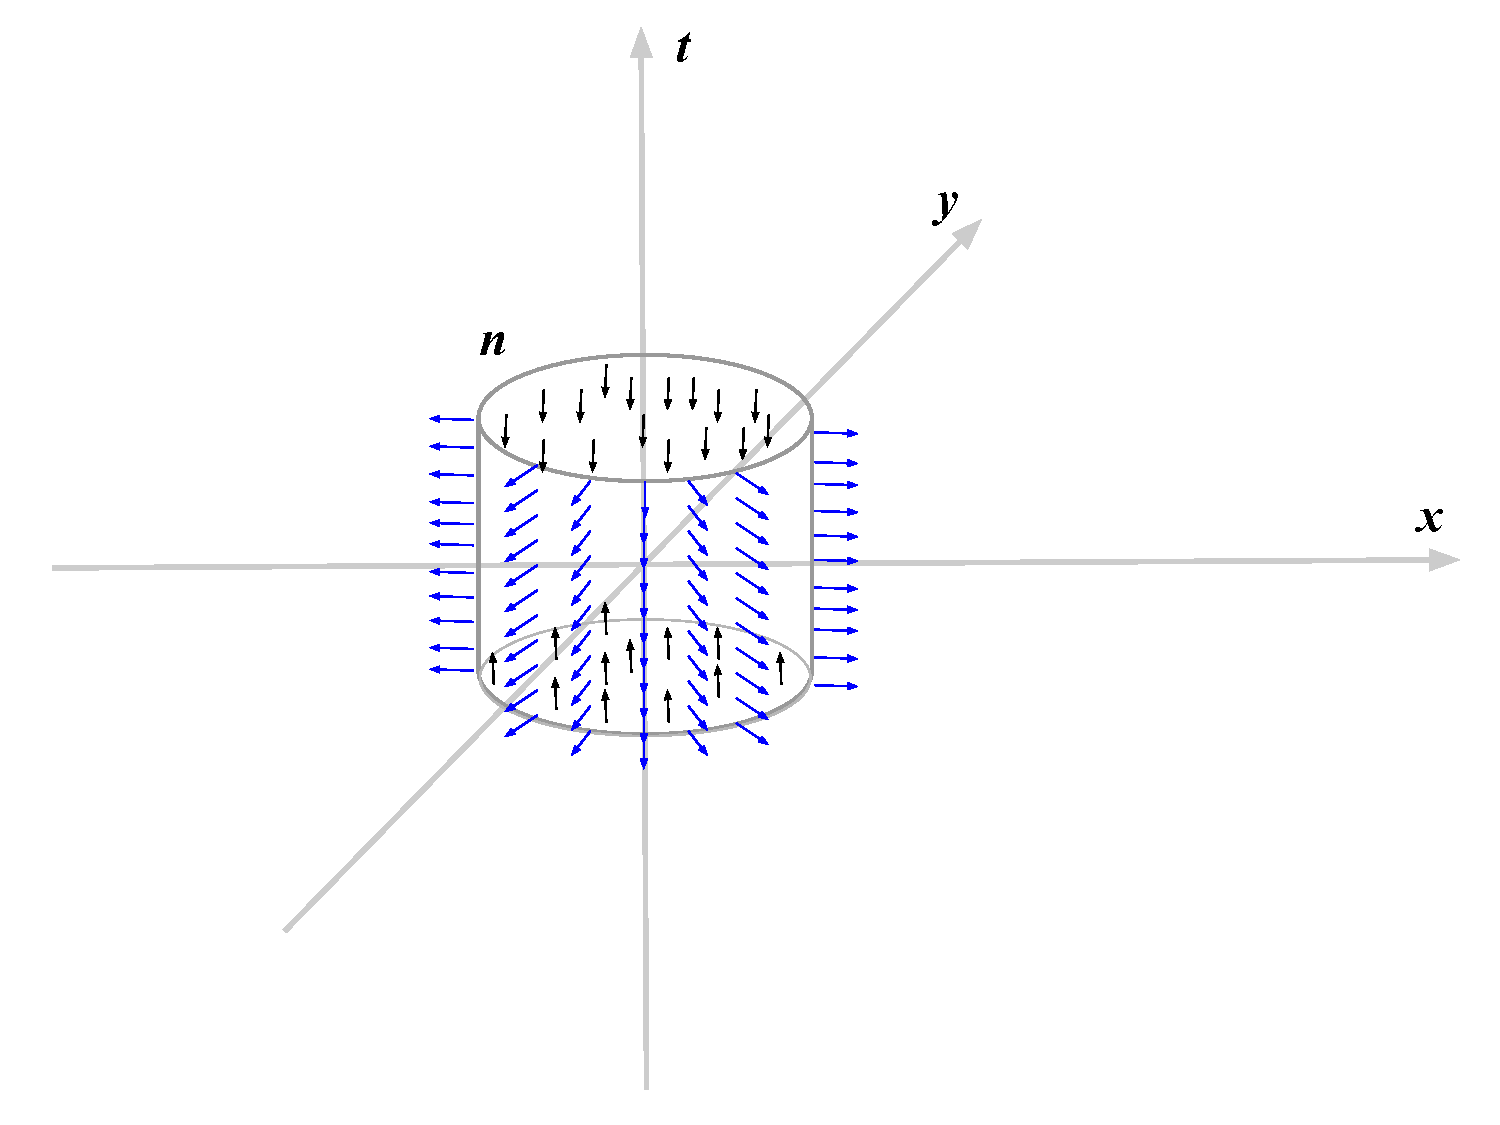
\includegraphics[scale=0.5]{figs/SpaceTimeNormal}
\caption{Normal vectors to the oriented surface in spacetime. Blue arrows indicate spacelike vectors. Black arrows indicate timelike vectors.}
\end{figure}
\subsection{Euler–Lagrange equation for Classic Field Theory}
Now we are ready to derive an equation (\ref{euler-lagrange-classic-field-I}) in the context of special relativity.
For a vector field $\phi^\alpha$, let's define an action functional as 
\begin{equation}
S(M, \phi^\alpha) := \int_M \mathcal{L}(\phi^\alpha, \partial_\mu \phi^\alpha, x^\mu) d^4x.
\end{equation}
We want to find a characteristic of a field $\phi^\alpha$, for which for any variation $\delta \phi^\alpha$ which vanishes at $\partial M$, we have
\begin{equation}
\delta S = 0.
\end{equation}
We assume that $\mathcal{L}$ is "nice enough" that we can go with $\delta$ under the integral. Thus we have:
\begin{equation}
\label{variation-under-integral-fields}
0 = \int_M \cfrac{\partial \L}{\partial \phi^\alpha} \delta \phi^\alpha + \cfrac{\partial \L}{\partial (\partial_\mu \phi^\alpha)} \delta \partial_\mu \phi^\alpha.
\end{equation}
Note that 
\begin{equation}
\label{for-partial-int-class-field}
\partial_\mu \bigg( \delta\phi^\alpha \cfrac{\partial \L}{\partial (\partial_\mu \phi^\alpha)}\bigg) = (\partial_\mu\delta\phi^\alpha)\cfrac{\partial \L}{\partial (\partial_\mu \phi^\alpha)}
+ \delta\phi^\alpha \partial_\mu \cfrac{\partial \L}{\partial (\partial_\mu \phi^\alpha)}.
\end{equation}
Since $\delta \phi^\alpha$ which vanishes at $\partial M$, by Theorem \ref{guass-theorem-relativistic}, we have
\begin{equation}
\int_M \partial_\mu \bigg( \delta\phi^\alpha \cfrac{\partial \L}{\partial (\partial_\mu \phi^\alpha)}\bigg) = \int_{\partial M} n_\mu \delta\phi^\alpha \cfrac{\partial \L}{\partial (\partial_\mu \phi^\alpha)} = 0.
\end{equation}
Thus by (\ref{for-partial-int-class-field}), we have
\begin{equation}
\label{fields-transposition}
\int_M (\partial_\mu\delta\phi^\alpha)\cfrac{\partial \L}{\partial (\partial_\mu \phi^\alpha)} = - \int_M \delta\phi^\alpha \partial_\mu \cfrac{\partial \L}{\partial (\partial_\mu \phi^\alpha)}.
\end{equation}
Since $\partial_\mu \delta \phi^a = \delta \partial_\mu \phi^a$ and by (\ref{variation-under-integral-fields}) and (\ref{fields-transposition}), we get
\begin{equation}
0 = \int_M \bigg(\cfrac{\partial \L}{\partial \phi^\alpha}  - \partial_\mu \cfrac{\partial \L}{\partial (\partial_\mu \phi^\alpha)}\bigg) \delta \phi^\alpha.
\end{equation}
Now, since $\delta \phi^\alpha$ is arbitrary, we get
\begin{equation}
\boxed{
\cfrac{\partial \L}{\partial \phi^\alpha}  - \partial_\mu \cfrac{\partial \L}{\partial (\partial_\mu \phi^\alpha)} = 0
}
\end{equation}
\section{Saturday, 10 November 2018}
Today, I am investigating various variational principles in special relativity classic field theory following \cite[17 The Classical Theory of Fields]{shepherd2013}
\subsection{Classical Field Theory -- Free particle with no field}
\label{classic-field-free-particle}
Let $x^\mu$ will be a curve which connects points in a spacetime $a$ and $b$. Assume that $b$ is "accessible" from $a$ and that we can paremetrise the curve by proper time $\tau$. Define an action along the curve as
\begin{equation}
S = -m\int_a^b d\tau.
\end{equation}
We are going to show that the above action is extremised by stright line in a spacetime. We will consider an arbitrary variation $\delta x^\mu$ which vanishes at $a$ and $b$.
\begin{equation}
\delta S = -m\delta\int_a^b d\tau = m\delta\int_a^b \sqrt{g_{\mu\nu} dx^\mu dx^\nu}. 
\end{equation}
Note that 
\begin{multline}
\delta F(f\cdot g) = F(f\cdot g) - F(f\cdot g + \delta(f\cdot g)) = (\delta f \cdot g + f \cdot\delta g)\dot{F}(f\cdot g).
\end{multline}
Thus
\begin{multline}
\delta S = -\cfrac{1}{2} m \int_a^b \cfrac{1}{\sqrt{g_{\mu\nu} dx^\mu dx^\nu}} g_{\mu\nu}(\delta dx^\mu dx^\nu + dx^\mu \delta dx^\nu)\\ = -m\int_a^b \cfrac{dx_\mu}{d\tau} \delta dx^\mu = -m\int_a^b u_\mu \delta dx^\mu = -m\int_a^b u_\mu d\delta x^\mu.
\end{multline}
Note that
\begin{equation}
d(u_\mu \delta x^\mu) = du_\mu \delta x^\mu + u_\mu d\delta x^\mu.
\end{equation}
Since $\delta x^\mu$ vanishes at $a$ and $b$, we have
\begin{equation}
\int_a^b du_\mu \delta x^\mu = -\int_a^b u_\mu d\delta x^\mu.
\end{equation}
And thus
\begin{equation}
\label{free-srt-action}
\delta S = m\int_a^b du_\mu \delta x^\mu = m\int_a^b \cfrac{du_\mu}{d\tau} \delta x^\mu d\tau.
\end{equation}
Since we require $\delta S = 0$ for arbitrary $\delta x^\mu$, we have
\begin{equation}
\boxed{
\cfrac{du_\mu}{d\tau} = 0}
\end{equation}
\subsection{Classical Field Theory -- Particle in a field with a vector potential}
Assume now that we have a vector potential $A_\mu$. We are now in the same context as in \ref{classic-field-free-particle}. The only difference is that we need to update action by the field-interacts-with-particle component. Let's define the action as
\begin{equation}
S = \int_a^b -md\tau + qA_\mu dx^\mu.
\end{equation}
By what was shown to get (\ref{free-srt-action}) we have
\begin{equation}
\label{vector-potential-started}
\delta S = \int_a^b mdu_\mu \delta x^\mu + q(\delta A_\mu dx^\mu + A_\mu \delta dx^\mu).
\end{equation}
Note that
\begin{equation}
d(A_\mu \delta x^\mu) = dA_\mu \delta x^\mu + A_\mu d\delta x^\mu.
\end{equation}
Since $\delta x^\mu$ vanishes in $a$ and $b$.
\begin{equation}
\int_a^b A_\mu d\delta A_\mu = -\int_a^b dA_\mu \delta x^\mu.
\end{equation}
Going back to \ref{vector-potential-started}, we get
\begin{equation}
\label{vector-potential-1}
\delta S = \int_a^b mdu_\mu \delta x^\mu + q(\delta A_\mu dx^\mu - dA_\mu \delta x^\mu).
\end{equation}
Let's calculate $\delta A_\mu$ and $dA_\mu$.
\begin{equation}
\delta A_\mu = \cfrac{\partial A_\mu}{\partial x^\nu}\delta x^\nu
\end{equation}
and
\begin{equation}
d A_\mu = \cfrac{\partial A_\mu}{\partial x^\nu}dx^\nu.
\end{equation}
Substitute the above in \ref{vector-potential-1}
\begin{equation}
\delta S = \int_a^b mdu_\mu \delta x^\mu + q(\cfrac{\partial A_\mu}{\partial x^\nu}\delta x^\nu dx^\mu - \cfrac{\partial A_\mu}{\partial x^\nu}dx^\nu \delta x^\mu).
\end{equation}
As summations in each part of the above equation is independent, we can exchange indecies in the 2nd part, i. e.
\begin{equation}
\delta S = \int_a^b mdu_\mu \delta x^\mu + 
q(\cfrac{\partial A_\nu}{\partial x^\mu}\delta x^\mu dx^\nu - \cfrac{\partial A_\mu}{\partial x^\nu}dx^\nu \delta x^\mu).
\end{equation}
Now
\begin{equation}
\delta S = \int_a^b \bigg( m \cfrac{du_\mu}{d\tau} 
+ q(\partial_\mu A_\nu - \partial_\nu A_\mu) u^\nu 
\bigg) \delta x^\mu d\tau.
\end{equation}
Since $\delta x^\mu$ is arbitrary and we require $\delta S = 0$, we get
\begin{equation}
\label{str-dynamics}
\boxed{
m \cfrac{du_\mu}{d\tau} = q(\partial_\nu A_\mu - \partial_\mu A_\nu) u^\nu
}
\end{equation}
Which is an equation of motion of a particle with charge $q$ and mass $m$ in a field with a vector potential $A_\mu$.
Let
\begin{equation}
F_{\nu\mu} := \partial_\nu A_\mu - \partial_\mu A_\nu.
\end{equation}
Note that from definition $F$ is antisymmetric, i.e. $F_{\mu \mu} = 0$ and $F_{\nu\mu} = - F_{\mu\nu}$. 
The equation (\ref{str-dynamics}) has now a form
\begin{equation}
\label{str-dynamics-F}
m \cfrac{du_\mu}{d\tau} = qF_{\nu\mu} u^\nu.
\end{equation}
Let's consider a particle $t\mapsto(\phi^0(t):= t, \phi^1(t), \phi^2(t), \phi^3(t))$ in a ceratain frame of refernce $x^\mu$.
Define
\begin{equation}
w^\mu := \frac{d\phi^\mu}{dt}.
\end{equation}
Note that $\vec{\omega} := (\omega^1, \omega^2, \omega^3)$ is an ordinary $3$-dimentional veliocity of the particle in the frame of referebnce $x^\mu$. Now assuming that covariant $4$-velocity of the particle is $u_\mu$ and recalling that $\frac{d\tau}{dt} = u_0^{-1}$, we may write an equation (\ref{str-dynamics-F}) is a form
\begin{equation}
m \cfrac{du_\mu}{dt} = qF_{\nu\mu}u^\nu u_0^{-1} = qF_{\nu\mu} \omega^\nu.
\end{equation}
Which translates into
\begin{equation}
\cfrac{dp_1}{dt} = q F_{01} + q(\omega^2 F_{21} - \omega^3 F_{13}).
\end{equation}
\begin{equation}
\cfrac{dp_2}{dt} = q F_{02} + q(\omega^3 F_{32} - \omega^1 F_{21}).
\end{equation}
\begin{equation}
\cfrac{dp_3}{dt} = q F_{03} + q(\omega^1 F_{13} - \omega^2 F_{32}).
\end{equation}
Now, if we put
\begin{equation}
\vec{E} := (F_{01}, F_{02}, F_{03})
\end{equation}
and
\begin{equation}
\label{rel_magnetic}
\vec{B} := (F_{32}, F_{13}, F_{21}).
\end{equation}
we get
\begin{equation}
\cfrac{d\vec{p}}{dt} = q\vec{E} + q\vec{\omega}\times \vec{B}.
\end{equation}
As a reference
\begin{equation}
F_{\nu\mu} = 
\begin{bmatrix}
0 & E_1 & E_2 & E_3 \\
-E_1 & 0 & -B_3 & B_2 \\
-E_2 & B_3 & 0 & -B_1 \\
-E_3 & -B_2 & B_1 & 0 \\
\end{bmatrix}.
\end{equation}
\section{Saturday, 17 November 2018}
\subsection{The Millikan Oil Drop Experiment}
Studing \textit{The Millikan Oil Drop Experiment} from \cite{melissinos-napolitano2003} and wrote a bit of python code for it
\begin{lstlisting}[language=Python, caption=How to calculate elementary charge from experiment data]
import numpy as np

mu = 1.849e-5
d = 7.63e-4
rho = 1.184 
sigma = 883
rho_prim = rho - sigma
g = 9.802 #New York Value
b = 6.17e-6
P = 76.01
V = 500
s = 4.71e-3

def _mu(a0, mu0=mu, P=P):
    return mu0 * ((1 + b/(a0*P))**-1)

def _a0(B, mu=mu):
    return ((9*B*mu*d)/(2*rho_prim*g))**0.5

def _e(A, a, mu):
    return (6*s*np.pi*a*mu*d*A)/V

B1 = [-27.9, -29.6, -28.2, -29.3, -29.4]

a = list(map(lambda B: _a0(1/B, _mu(_a0(1/B))), B1))
better_a = np.array(a).mean()
better_mu = _mu(better_a, mu)
\end{lstlisting}
\section{Saturday, 8 December 2018}
\subsection{Classical picture for studing Einstein-de Haas effect.}
\begin{figure}[H]

\centering
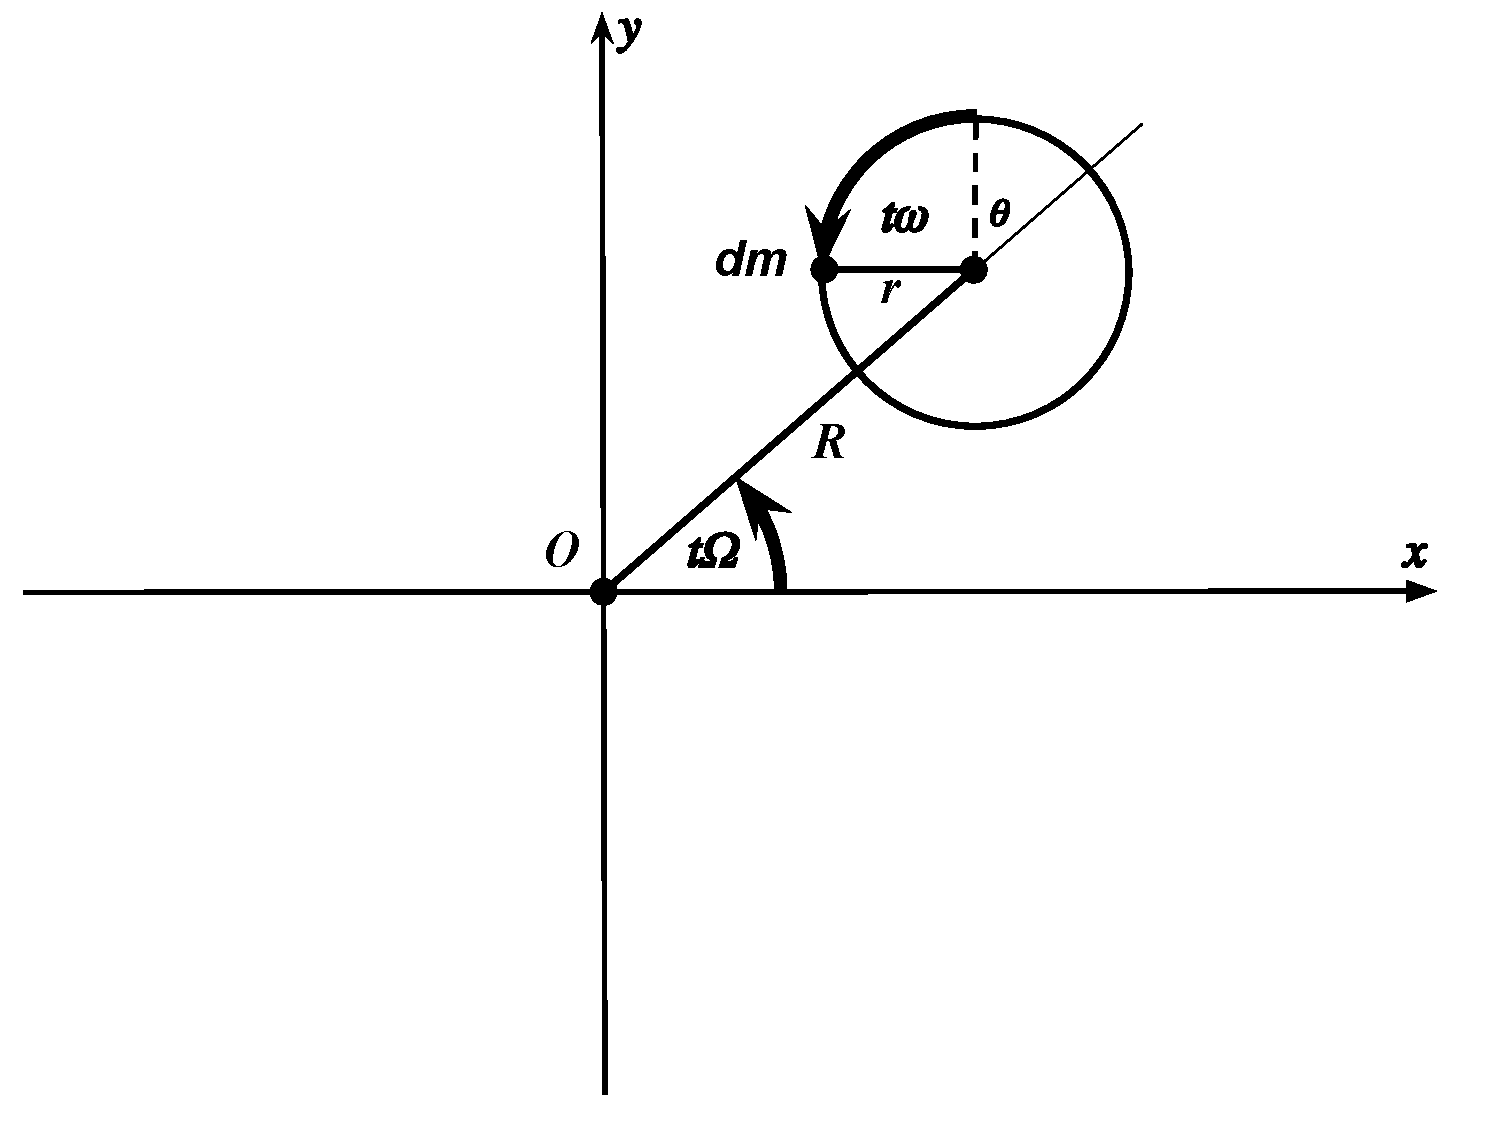
\includegraphics[scale=0.5]{figs/Angular}
\caption{A circular hoop rotating around its center, which itself rotate around the central point $O$.}
\label{fig:hoop}
\end{figure}
Our goal will be to calculate an angular momentum $\vec{L}$ (relative to the central point $O$) of a system consisting of a circular hoop rotating around its center, which itself also rotates around the central point $O$.

Assume that the circular hoop (lying is a plane $xy$) has a mass $m$ and radious $r$, it's rotating around its center (axis of rotation perpendicular to the plane $xy$), which is fixed at one end of an arm of length $R$ (lying in the plane $xy$) which again rotates with angular velocity $\Omega$ around its other end $O$ in a plane of the hoop. Moreover assume that circular hoop rotates with an angular velocity $\omega$ relative to the arm. The situation is symbolically pictured on Figure \ref{fig:hoop}).

Assume that at the moment $t=0$ the center of the hoop was in the point $(R, 0)$.
Consider an infinitesimal element of the hoop $dm$ which at the moment $t=0$ was at an angle $\theta$ to the extention of the arm (marked on Figure \ref{fig:hoop}). We may assume that $dm = \rho d\theta$ where $\rho$ is a constant angular density of the hoop. Let $\vec{q}_\theta(t)$ dentote position of the infinitesimal element of the hoop in time t.
\begin{equation}
\vec{q}_\theta(t) = (Rcos(t\Omega) + rcos(t\omega + \theta + t\Omega), Rsin(t\Omega) + rsin(t\omega + \theta + t\Omega),0)
\end{equation}
The angular momentum $d\vec{L}$ of the infinitesimal element of the hoop is equal to:
\begin{equation}
d\vec{L} = \vec{q}_\theta \times dm \dot{\vec{q_\theta}}.
\end{equation}
After simplifications done by Mathematica 11.3 (\cite{mathematica2018}).

\begin{doublespace}
\noindent\(\pmb{\alpha [\text{t$\_$}]\text{:=}\Omega  *t }\\
\pmb{\beta [\text{t$\_$}] \text{:=} \omega *t}\\
\pmb{\theta [\text{t$\_$}]\text{:=}\alpha [t]-\beta [t]}\\
\pmb{x[\theta \_,\text{t$\_$}] \text{:=} \{R*\text{Cos}[\alpha [t]] + r*\text{Cos}[\alpha [t] + \beta [t]+\theta ],}\\
\pmb{R*\text{Sin}[\alpha [t]] + r*\text{Sin}[\alpha [t] + \beta [t]+\theta ],0\}}\\
\pmb{\text{xdot}[\theta \_,\text{t$\_$}] \text{:=} D[x[\theta ,t], t]}\\
\pmb{\text{TrigReduce}[ x[\theta , t]\times \text{xdot}[\theta , t]]}\)
\end{doublespace}

\begin{doublespace}
\noindent\(\left\{0,0,r^2 \omega +r^2 \Omega +R^2 \Omega +r R \omega  \text{Cos}[\theta +t \omega ]+2 r R \Omega  \text{Cos}[\theta +t \omega ]\right\}\)
\end{doublespace}
\begin{equation}
d\vec{L} = \rho d\theta\big(0, 0, r^2(\omega + \Omega) + R^2\Omega + (rR\omega + 2rR\Omega)cos(\theta + t\omega)\big). 
\end{equation}
Now 
\begin{equation}
\vec{L} = \int_0^{2\pi} d\vec{L} = \big(0, 0, mr^2(\omega + \Omega) + mR^2\Omega\big).
\end{equation}
Let $\omega'$ be an angular velocity of the hoop relative to the plane $xy$, then $\omega' = \omega + \Omega$. Asumme that $\vec{L} = (L_x, L_y, L_z)$. Thus $L_x = L_y = 0$ and
\begin{equation}
\label{summary_angular_momentum}
L_z = mr^2\omega' + mR^2\Omega.
\end{equation}
Assume now that we have a crystal structure in a shape of a cylindrical bar located perpendicularly to the plane $xy$ with its hight parallel to $z-axis$. The bar rotates with an angular velocity $\Omega$ around its symmetry axis which lies along $z-axis$. Assume that the crystal structure has $N$ nodes indexed from $1$ to $N$, where $\Delta m$ is a mass of each node. Assume that each node is a small hoop (lying in the plane parallel to $xy$ plane) of some small radius $r$, rotating around its center with an angular velocity $\omega_i'$ (relative to plane $xy$) in a plane parallel to $xy$ plane (axis of rotation goes through the center of the hoop and is perpendicular to the plane $xy$).
From this point $\vec{L} = (L_x, L_y, L_z)$ will denote a total angular momentum of the crystal structure (relative to $z-axis$).
Let $\vec{L}_i = (0, 0, \Delta mr^2\omega_i')$ be an ``intristic'' 
angular momentum of $i-th$ node (as if ignoring the movement of its center due to the rotation of the bar). Let $R_i$ be a distance of $i-th$ node from the bar's rotation axis.

By (\ref{summary_angular_momentum}) we have that total angular momentum of the bar is
\begin{equation}
L_z = \sum_{i=1}^N (L_i)_z + \sum_{i=1}^N \Delta mR_i^2\Omega = \sum_{i=1}^N (L_i)_z + \Omega \sum_{i=1}^N \Delta mR_i^2.
\end{equation}
Thus
\begin{equation}
\vec{L} = \sum_{i=1}^N \vec{L}_i + \Omega \vec{I},
\end{equation}
where $\vec{I}$ is a moment of inertia of the solid cylinder of the shape of our cylindrical bar and exactly the same mass.
\section{Thursday, 20 December 2018}
\subsection{Lifetime of excited states in Hydrogen}
Reviewing Schrödinger model of hydrogen atom, I was also considering theoretical ways to calculate lifetimes of excited states. I have found an interesting paper \cite{verolainen_nikolaich1982} from 1982 which summarises theoretical and experimental results up to date. It is a valuable source of references.
Also key word here is: Fermi's golden rule.
\section{Sunday, 27 January 2019}
\subsection{Momentum conservation in the quantum two-body problem}
\label{QM-momentum-conservation-2body}
In this subsection, we will work with Planck units.
Consider Schrödinger equation of two particles, where interaction depends only on the distance between them. 
\begin{equation}
i\cfrac{\partial \psi}{\partial t} = H\psi,
\end{equation}
where
\begin{equation}
\label{two-body-hamiltonian}
H\psi = \cfrac{P^2_x}{2m_x}\psi + \cfrac{P^2_y}{2m_y}\psi + V(x-y)\psi. 
\end{equation}
and where $\psi$ depends on $(t, x, y)$ and $x=(x_1, x_2, x_3), y=(y_1, y_2, y_3)$.
\begin{equation}
P^2_x := P^2_{x,1} + P^2_{x,2} + P^2_{x,3},
\end{equation} 
where 
\begin{equation}
P_{x,i} := -i\cfrac{\partial}{\partial x_i},
\end{equation}
and
\begin{equation}
P^2_y := P^2_{y,1} + P^2_{y,2} + P^2_{y,3},
\end{equation} 
where 
\begin{equation}
P_{y,i} := -i\cfrac{\partial}{\partial y_i}.
\end{equation}
We are going to prove that
\begin{equation}
\label{quantum-mechanics-momentum-conservation}
[P_{x,i} + P_{y,i}, H] = 0.
\end{equation}
Let's calculate 
\begin{multline}
\label{momentum-and-potential-symultanious-measurment}
(P_{x,i} + P_{y,i})(V(x-y)\psi) = \\
-i\dot{V}(x - y)\psi + V(x - y)P_{x,i}\psi +  
(-i)(-\dot{V}(x - y))\psi + V(x - y)P_{y,i}\psi \\
= V(x - y)(P_{x,i} + P_{y,i})\psi. \\
\\
\end{multline}
On the other hand it's obvious that 
\begin{equation}
\label{momentum-and-kinetic-symultanious-measurment}
[P_{x,i} + P_{y,i}, \cfrac{P^2_x}{2m_x} + \cfrac{P^2_y}{2m_y}] = 0.
\end{equation}
Thus by (\ref{momentum-and-potential-symultanious-measurment}) and (\ref{momentum-and-kinetic-symultanious-measurment}), we have (\ref{quantum-mechanics-momentum-conservation}).

Found an interesting paper on two-body problem in quantum mechanics \cite{micu-hulubei2008}.
\section{Saturday, 23 February 2019}
\subsection{Reduced mass in Quantum Mechanics}
\label{reduced-mass-in-quantum}
In this subsection we will continue to work with Hamiltonian introduced in \ref{two-body-hamiltonian} and with annotations introduced in Subsection \ref{QM-momentum-conservation-2body}.
Let's introduce new system of coordinates
\begin{equation}
\begin{cases}
R := \cfrac{m_x}{m_x + m_y}x + \cfrac{m_y}{m_x + m_y}y,\\
r := x - y. 
\end{cases}
\end{equation}
We can now express $\psi$ in $t,r,R$. $R$ is a position of mass centre and $r$ is a vector between two positions $x,y$.
Check that
\begin{equation}
\begin{cases}
x = R + \cfrac{m_y}{m_x + m_y}r,\\
y = R - \cfrac{m_x}{m_x + m_y}r,
\end{cases}
\end{equation}
Define operators
\begin{equation}
P_{r,i}:= -i\cfrac{\partial}{\partial r_i}.
\end{equation}
and
\begin{equation}
P_{R,i}:= -i\cfrac{\partial}{\partial R_i}.
\end{equation}
Note that
\begin{equation}
\cfrac{\partial \psi}{\partial r_i} = \cfrac{\partial \psi}{\partial x}
\cfrac{\partial x}{\partial r_i} + \cfrac{\partial \psi}{\partial y}
\cfrac{\partial y}{\partial r_i} =  \cfrac{m_y}{m_x + m_y}\cfrac{\partial \psi}{\partial x_i} - \cfrac{m_x}{m_x + m_y}\cfrac{\partial \psi}{\partial y_i}. 
\end{equation}
Thus
\begin{equation}
P_{r,i} = \cfrac{m_y}{m_x + m_y}P_{x,i} - \cfrac{m_x}{m_x + m_y}P_{y,i}.
\end{equation}
On the other hand
\begin{equation}
P_{R,i} = P_{x,i} + P_{y,i}.
\end{equation}
Let
\begin{equation}
M = m_x + m_y,
\end{equation}
which is total mass of the system and
\begin{equation}
\mu = \cfrac{m_xm_y}{m_x + m_y},
\end{equation}
which is reduced mass.
Next, note that
\begin{equation}
\cfrac{P^2_{r,i}}{2\mu} = \cfrac{m_y}{2m_x(m_x+m_y)}P^2_{x,i} - \cfrac{1}{m_x+m_y}P_{x,i}P_{y,i} + \cfrac{m_x}{2m_y(m_x+m_y)}P^2_{y,i}.
\end{equation}
On the other hand
\begin{equation}
\cfrac{P^2_{R,i}}{2M} = \cfrac{1}{2(m_x+m_y)}(P^2_{x,i} + 2P_{x,i}P_{y,i} + P^2_{y,i}).
\end{equation}
Note that
\begin{equation}
\cfrac{m_y}{2m_x(m_x+m_y)} + \cfrac{1}{2(m_x+m_y)} = \cfrac{1}{2m_x},
\end{equation}
and
\begin{equation}
\cfrac{m_x}{2m_x(m_x+m_y)} + \cfrac{1}{2(m_x+m_y)} = \cfrac{1}{2m_y}.
\end{equation}
Thus, eventually we get
\begin{equation}
\cfrac{P^2_{r,i}}{2\mu} + \cfrac{P^2_{R,i}}{2M} = \cfrac{P^2_x}{2m_x} + \cfrac{P^2_y}{2m_y}.
\end{equation}
Thus if we introduce two hamiltonians:
\begin{equation}
H_r \psi = \cfrac{P^2_{r,i}}{2\mu}\psi + V(r)\psi,
\end{equation}
and
\begin{equation}
H_R \psi = \cfrac{P^2_{R,i}}{2M},
\end{equation}
we will get
\begin{equation}
H = H_r + H_R.
\end{equation}
It is crucial to note at this point that if we look at $\psi$ as dependent on $t,r,R$, $H_r$ acts seperately on coordinate $r$ and $H_R$ acts seperately on coordinate $R$ and that $P_{r,i}$ and $P_{R,i}$ are respectively momentum operators.

Thus we might find solution of stationary equation $H\psi = E\psi$ by $\psi(r,R) = \phi_1(r)\phi_2(R)$, where $H_r\phi_1 = E_r\phi_1$ and $H_R\phi_2 = E_R\phi_2$.
\section{Thursday, 16 May 2019}
\subsection{The electromagnetic field as an infinite system of harmonic oscilators}

The idea of continuum limit of harmonic oscilators is mentioned in \cite[5.3]{lancaster-blundell2018}. It is described in details in \cite[see][6 Quantization of the Electromagnetic Field]{dauria-trigiante2012}.

Non-relativistic probability current in Quantum Mechanics, mentioned in \cite[6.2 Probability currents and densities]{lancaster-blundell2018} is introduced e.g. in \cite[3.6 Probability conservation]{desai2010}.

\section{Sunday, 26 May 2019}
\subsection{Derivation of the Schrödinger equation from the Ehrenfest theorems}
Through wikipedia's entry on Ehrenfest theorem \cite[see e.g.][3.7]{desai2010}, I have found a paper \cite{bondar2012} in which authors shows how to derive Schrödinger equation from the thesis of Ehrenfest theorem. The key point is the use of canonical comutation between momentum and position operators. It is showed as well that if the operators commute, we get Koopman–von Neumann classical mechanics. Recently they managed to generalise their result to Dirac Equation in \cite{cabrera2019}.
\subsection{Ehrenfest theorem}
Assume that $\psi(t)$ is a solution of Schrödinger equation
\begin{equation}
i\hbar \cfrac{d \psi}{d t}(t) = H\psi(t).
\end{equation}
Consider observalble $A$ which is composed of momentum and position operators.
\begin{equation}
\label{ehrenfest-calc-1}
i\hbar \cfrac{d}{d t}(\psi(t), A\psi(t)) = (i\hbar \cfrac{d \psi}{d t}(t), A\psi(t)) - (\psi(t), i\hbar \cfrac{d}{d t} A\psi(t))
\end{equation}
As $A$ is composed of momentum and position operators, it is clear that it comutes with $\cfrac{d}{d t}$, thus we may continue the equation \ref{ehrenfest-calc-1} as follows:
\begin{multline}
\\(i\hbar \cfrac{d \psi}{d t}(t), A\psi(t)) - (\psi(t), Ai\hbar \cfrac{d}{d t}\psi(t)) = 
\\ (H\psi(t), A\psi(t)) - (\psi(t), AH\psi(t)) =
\\(\psi(t), HA\psi(t)) - (\psi(t), AH\psi(t)) = 
\\(\psi(t), (HA - AH)\psi(t)) = (\psi(t), [H,A]\psi(t)).
\\
\end{multline}
In bra-ket notation:
\begin{equation}
\label{ehrenfest-physic}
i\hbar \cfrac{d}{d t} \mel{\psi(t)}{A}{\psi(t)} = \mel{\psi(t)}{[A,H]}{\psi(t)}.
\end{equation}
Assume that we have hamiltonian 
\begin{equation}
H = \sum_{i=0}^3 \cfrac{P_i^2}{2m} + V(Q_1,Q_2,Q_3).
\end{equation}
Note that
\begin{equation}
[Q_i, H] = \cfrac{1}{2m}[P_i^2, Q_i] = \cfrac{i\hbar P_i}{m}.
\end{equation}
Thus by \ref{ehrenfest-physic}
\begin{equation}
\cfrac{d}{d t} \mel{\psi(t)}{Q_i}{\psi(t)} = \cfrac{1}{m}\mel{\psi(t)}{P_i}{\psi(t)}.
\end{equation}
Note that
\begin{equation}
[P_i, H] = [P_i, V] = -i\hbar \cfrac{\partial V}{\partial x_i}. 
\end{equation}
Thus by \ref{ehrenfest-physic}
\begin{equation}
\cfrac{d}{d t} \mel{\psi(t)}{P_i}{\psi(t)} = \mel{\psi(t)}{-\cfrac{\partial V}{\partial x_i}}{\psi(t)}.
\end{equation}
\section{Monday, 27 May 2019}
\subsection{Hamiltonian of electromagnetic field}
The hamiltonian is itroduced without proof in \cite[6.2]{desai2010}. The deriviation can be found in \cite[Examples 9.1 and 9.2]{walter-greiner2001}.
\section{Tuesday, 28 May 2019}
\subsection{Interaction with the orbital angular momentum}
In \cite[6.5]{desai2010}, we need to assume $\vec{B} = \text{const}$, to have $A = \cfrac{1}{2}(\vec{B}\times\vec{r})$ and $\nabla\times A = B$.
\section{Tuesday, 2 July 2019}
\subsection{Dirac Delta Function in the Context of Fourier Transform in Physical Texts}
We will calculate Fourier Transform (as defined in Definition \ref{multi-fourier-transform}) of $1$ understood as distribution.

\begin{multline}
\\
\F(1)(\phi) = 1(\F(\phi)) = \int_{\reals^n} \F(\phi) \cdot 1 = \int_{\reals^n} \F(\phi) \cdot e^{ix\cdot 0} dx = \\
(2\pi)^\frac{n}{2}\F^{-1}(\F(\phi))(0) = (2\pi)^\frac{n}{2}\phi(0).\\
\end{multline}
Thus from the definition of Dirac delta-function understood as distribution
\begin{equation}
\boxed{
\label{dirac-delta-as-one-distribution}
\F(1) = (2\pi)^\frac{n}{2}\delta_0. 
}
\end{equation}
Equivalently 
\begin{equation}
\delta_0 = (2\pi)^{-\frac{n}{2}}\F(1).
\end{equation}
Let's calculate now Fourier Transform of Dirac delta:
\begin{multline}
\F(\delta_0)(\phi) = \delta_0 (\F(\phi)) = \F(\phi)(0) =  \int_{\R^n} \phi(x) e^{-ix\cdot 0}dx = \\
(2\pi)^{-\frac{n}{2}} \int_{\R^n} \phi(x) \cdot 1 dx =  (2\pi)^{-\frac{n}{2}} 1(\phi).
\\
\end{multline}
Thus
\begin{equation}
\boxed{
\label{fourier-delta}
\F(\delta_0) = (2\pi)^{-\frac{n}{2}} \cdot 1.
}
\end{equation}
If we apply inverse Fourier transform to the equation (\ref{fourier-delta}), we obtain
\begin{equation}
\label{dirac-delta-as-inv-one-distribution}
\delta_0 = (2\pi)^{-\frac{n}{2}}\F^{-1}(1).
\end{equation}
From equations (\ref{dirac-delta-as-one-distribution}) and (\ref{dirac-delta-as-inv-one-distribution}) it is apparent that
\begin{equation}
\F(1) = \F^{-1}(1)
\end{equation}
and
\begin{equation}
\F(\delta_0) = \F^{-1}(\delta_0),
\end{equation}
which is intuitive as both distributions are symmetric.
In physics texts (e.g. \cite{thomson2016}), equations such as the equation (\ref{dirac-delta-as-inv-one-distribution}) are usually written as
\begin{equation}
\\
\delta(k) = (2\pi)^{-n}\int_{\R^n} e^{ikx}dx,\\
\end{equation}
despite the fact that the integral $\int_{\R^n} e^{ikx}dx$ doesn't exist in classical measure theory sense. If one knows distribution theory, it is easy to understand that the meaning of this is symbolic and has certain algebraic sense, however not experienced reader might encounter great dificulties, when one sees such an intergral for the first time without necessery commentary.

For distribution theory see e.g \cite[Distributions and Fourier Transforms]{rudin1991} or \cite[3.3 Distributions]{miklavcic1998}.
\section{Saturday, 3 August 2019}
\subsection{Futher investigation in mathematical rigor in Dirac notation}

My problem is that physists use equations like
\begin{equation}
\braket{\psi_\alpha}{\psi_\beta} = \delta(\alpha - \beta),
\end{equation}
even where $\int \psi_\alpha^* \psi_\beta$ isn't defined properly. As I understand, this requires to see at least the mapping $\alpha \mapsto \braket{\psi_\alpha}{\psi_\beta}$ not as a function but distribution. Thus definition of $\braket{\psi_\alpha}{\psi_\beta}$ can't be any longer $\int \psi_\alpha^* \psi_\beta$ in terms of integral over complex functions.

As I understand the proper mathematical rigor is achived through rigged Hilbert spaces. The nice summary of mathematics basis for Dirac formalism is here \cite{gadella2003} also a good strating point is \cite{madrid2005}.

I tried to make a shortcut, because in lucky case we can easily understand $\alpha\mapsto \braket{\psi_\alpha}{\psi_\beta}$ as distribution for $\psi_\alpha(x) = e^{-i\alpha\cdot x}$ as Fourier transform extended on the space of tempered distribution, I was thinking about the following generalisation:

\begin{theorem}
\label{continous-basis-helper}
Let $\{u_\alpha\}_{\alpha\in\R^n} \subset S'_n$. If a transformation $\T_u$ defined as
\begin{equation}
(\T_u(\phi))(\alpha) = u_\alpha(\phi) \text{ for } \phi\in S_n \text{ and } \alpha\in\R^n
\end{equation}
is a continuous mapping $\T_u:S_n\to S_n$, then the transformation $\hat{\T_u}$ defined as
\begin{equation}
\hat{\T_u}(v)(\phi) = v(\T_u(\phi)) \text{ for } v\in S_n' \text{ and } \phi\in S_n, 
\end{equation}
is a continuous mapping $\hat{\T_u}:S_n'\to S'_n$ in $S_n'$ with weak* topology.
\end{theorem}
\begin{proof}
This version or very similiar should be proved. Not done yet.
\end{proof}

However, even if above theorem is true, it doesn't solve the main issue because opposite to the special case of Fourier transform, transformation $\hat{\T_u}$ in general case is not an extension of $\T_u$ in sense of $S_n\subset S_n'$ (when we consider functions from $S_n$ as distributions).

Now I will try to study if I can't achive something similiar using integral in space of measurable functions into the space of distribuitions. But most likely this aproach will be not successul as Schwartz showed that multiplication of distributions is not associative (\cite[see][XIX. Theory of Distributions 7. Operations of distributions]{maurin1980})
\subsection{Plan for rigorous theory which includes Dirac notation}
\label{dirac-plan}
We will need a notion of integral of distribution $u\in\D'(\R^n)$
\begin{equation}
\int_A u d\mu
\end{equation}
defined as some kind of limit $\lim_{n\to \infty}u(\psi_n)$ where $D(\R^n)\ni\psi_n\to 1_A$ in certain sense.
With this kind of definition we will have
\begin{equation}
\int_{\R^n} \delta_z dx = 1,
\end{equation} 
for any $z\in\R^n$, where $\delta_z$ is Dirac delta in point $z$.
We will also need to define the integral of functions with values in the space of distributions. Something like that:
\begin{definition}
\label{def-vector-integral-for-distributions}
Let $\Omega$ be an open subset of $\R^k$ and 
let $\mu$ be any Borel measure on $\Omega$ and let $A$ be any borel set. Let $u:A\to\D'(\R^k)$ be a function for which a function $A\ni \alpha\mapsto u_\alpha(\psi)$ is measurable for any $\phi\in \D(\Omega)$. We will call such $u$ measurable. We define that 
\begin{equation}
\label{vector-integral-for-distributions}
\int_A u_\alpha d\mu(\alpha):= v
\end{equation}
iff $v\in \D'(\Omega)$ and 
\begin{equation}
v(\phi) = \int_A u_\alpha(\phi) d\mu(\alpha) \text{ for any } \phi\in \D(\Omega).
\end{equation}
We say that the integral from (\ref{vector-integral-for-distributions}) exists if there exists such a $v$.   
\end{definition}

Note that with this setup for any measurable function $f:A\to \C$ the integral $\int_A f(\alpha)u_\alpha d\mu(\alpha)$ has sense, as we treat $f(\alpha)$ as scalar value by which we multiply distribution $u_\alpha$.

When in our considerations we treat distributions $\D'(\Omega)$ as vectors, the equivalent of matrix are distributions $\D'(\Omega\times\Omega)$. In that sense we might want to concatenate values of $u:\Omega\to\D'(\Omega)$ into matrix $U\in \D'(\Omega\times\Omega)$. In order to do that we introduce operation $(.)_{\alpha\in\Omega}$.

\begin{definition} (\textbf{Generalised matrix})
\label{generalised-matrix}
Let $\Omega$ be an open subset of $\R^k$ and $u:\Omega\to\D'(\Omega)$ 
be Borel measurable. We define
\begin{equation}
(u_\alpha)_{\alpha\in\Omega} := U
\end{equation}
iff $U\in\D'(\Omega\times\Omega)$ and
\begin{equation}
U(\phi) = \int_\Omega u_\alpha(\phi(\alpha, \cdot))d\alpha,
\end{equation}
for any $\phi\in \D(\Omega\times\Omega)$.
We say that $(u_\alpha)_{\alpha\in\Omega}$ exists if there is such $U$.
\end{definition}

For any function $f:A\times B \to C$ defined on the product of sets, we can define transposition as $f^T:B\times A \to C$ such that $f^T(b, a) = f(a,b)$ for any $a\in A$ and $b\in B$. Note that for any $\phi\in\D(\Omega\times\Omega)$, we have $\phi^T\in\D(\Omega\times\Omega)$.

\begin{definition} (\textbf{Generilised transposition})
Let $\Omega$ be an open subset of $\R^k$ and let $U\in \D'(\Omega\times\Omega)$. We define a transposition of $U$ as $U^T\in \D'(\Omega\times\Omega)$ such that
\begin{equation}
U^T(\phi) := U(\phi^T) \text{ for any } \phi\in\D(\Omega\times\Omega).
\end{equation}
\end{definition}
In this terms for any measurable $\Omega\ni\alpha \mapsto u_\alpha\in\D'(\Omega)$ and $\psi\in C^\infty(\Omega)$ we can define Dirac bra-ket understood as a distribution with domain indicated by argument $\alpha$ 
\begin{equation}
\braket{\psi}{u_\alpha} := \int_{\Omega} \psi(\beta)^* u^\beta d\alpha.
\end{equation} where $\Omega\ni\beta\mapsto u^\beta\in\D'(\Omega)$ is a measurable function such that $(u^\beta)_{\beta\in\Omega} = \big((u_\alpha)_{\alpha\in\Omega}\big)^T$, provided that the integral exists.
Next we can extend this as
\begin{equation}
\braket{v}{u_\alpha} := \lim_{n\to\infty} \braket{\psi_n}{u_\alpha},
\end{equation}
if the above limit (understood in $\D'(\Omega)$ with weak-* topology) exists and is the same for any $\D(\Omega)\psi_n\to v$ in $\D'(\Omega)$ with weak-* topology.\\
Note that if $\alpha\to \braket{v}{u_\alpha}$ happen to be a function, each complex value $\braket{v}{u_\alpha}$ has sense for any $\alpha$. Thus this definition defines Dirac bra-kets as scalars whenever they have sense as scalars. It is possible that for this all to work additional condition that $u_\alpha$ is in certain sense orthogonal basis might be required.

There is a channce this construction will evolve into generalised vector spaces with vectors generelised to measures with notation $\int_A f(\alpha)u_\alpha d\mu(\alpha)$ which unifies finite and infinite dimension vector spaces.

When we will write $\braket{v}{u_\alpha}$ in the context of distribution, it will always mean distribution with the domain indicated by the index in bra.
\begin{remark}
If we are in the context of tempered distributions, we need to replace $\D(\Omega)$ by $S_k$, $\D'(\Omega)$ by $S_k'$, $\D(\Omega\times\Omega)$ by $S_{2k}$ and $\D'(\Omega\times\Omega)$ by $S'_{2k}$ in the above definitions.  
\end{remark}
\section{Sunday, 18 August 2019}
\subsection{Rigorous Dirac Formulation}
We will continue considerations that we bagan in subsection \ref{dirac-plan}. We will use dirac delta $\delta_\alpha$ as defined in Definition \ref{dirac-delta}.
We will also define
\begin{definition}
Let $\alpha\in\R^k$. Let's define $e_\alpha:\R^k\to \C$ as
\begin{equation}
e_\alpha(x) = (2\pi)^{-\frac{k}{2}} e^{-i\alpha \cdot x}.
\end{equation}
By Example \ref{exponent-tempered} we can treat $e_\alpha$ as an element of $S'_k$.
\begin{fact} Let $\alpha\in\R^k$, then
$\F(\delta_\alpha) = e_\alpha$.
\end{fact}
\begin{proof}
\begin{equation}
\F(\delta_\alpha)(\phi) = \delta_\alpha(\F(\phi)) = \F(\phi)(\alpha) = \int e_\alpha \phi = e_\alpha(\phi)
\end{equation}
for any $\phi \in S_n$.
\end{proof}
\begin{fact}
Let $\alpha\in\R^k$, then $\F(e_\alpha) = \delta_{-\alpha}$.
\end{fact}
\begin{proof}
\begin{equation}
\F(e_\alpha)(\phi) = e_\alpha(\F(\phi)) = \int e_\alpha \F(\phi) = \phi(-\alpha) = \delta_{-\alpha}(\phi)
\end{equation}
for any $\phi \in S_n$.
\end{proof}
\begin{proposition}
$(\delta_\alpha)_{\alpha\in\R^k} = \big((\delta_\alpha)_{\alpha\in\R^k} \big)^T$.
\end{proposition}
\end{definition}
\begin{proof}
Let $U = (\delta_\alpha)_{\alpha\in\R^k}$. Note that by Definition \ref{generalised-matrix} $U(\phi) = \int \phi(\alpha,\alpha) d\alpha$. Thus $U^T = U$.  
\end{proof}
\begin{proposition}
$(e_\alpha)_{\alpha\in\R^k} = \big((e_\alpha)_{\alpha\in\R^k} \big)^T$.
\end{proposition}
\begin{proof}
Let $U = (e_\alpha)_{\alpha\in\R^k}$. By Definition \ref{generalised-matrix} 
\begin{equation}
U(\phi) = (2\pi)^{-\frac{k}{2}} \int \int e^{-i\alpha \cdot \beta} \phi(\alpha, \beta) d\alpha d\beta .
\end{equation}
Thus $U^T = U$.
\end{proof}
\begin{definition}
Let $\Omega$ be an open subset of $\R^k$.
Define $(.)^*:D'(\Omega)\to D'(\Omega)$ as
\begin{equation}
u^*(\phi) := (u(\phi^*))^*,
\end{equation}
where $u\in D'(\Omega)$ and $\phi\in D(\Omega)$. 
\end{definition}
\begin{corollary}
$(.)^*:D'(\Omega)\to D'(\Omega)$ is continuous in $\D'(\Omega)$ with weak-* topology.
\end{corollary}
\begin{corollary}
$\delta_\alpha^* = \delta_\alpha$ for any $\alpha\in\R^k$.
\end{corollary}
\begin{corollary}
$e_\alpha^* = e_{-\alpha}$ for any $\alpha\in\R^k$.
\end{corollary}
\begin{theorem}
If $u\in \D'(\R^k)$, then
\begin{equation}
\braket{u}{\delta_\alpha} = u^*.
\end{equation}
\end{theorem}
\begin{proof}
Take any $D(\R^k)\ni f_n \to u$ in $\D'(\R^k)$ with weak-* topology.
We should have
\begin{equation}
\braket{f_n}{\delta_\alpha} = \int f^*_n(\alpha) \delta_\alpha d\alpha.
\end{equation}
Take any $\phi\in\D'(\R^k)$.
\begin{equation}
\int f^*_n(\alpha) \delta_\alpha(\phi) d\alpha = \int f^*_n(\alpha)\phi(\alpha) d\alpha \to u^*(\phi).
\end{equation}
Thus $\braket{f_n}{\delta_\alpha} = f^*_n \to u^*$. 
\end{proof}
The above proof could be easily modified to give the following:
\begin{theorem} (In the context of tempered distributions)
If $u\in S'_n$, then
\begin{equation}
\braket{u}{\delta_\alpha} = u^*.
\end{equation} 
\end{theorem}
\begin{corollary}
$\braket{\delta_\beta}{\delta_\alpha} = \delta_\beta$.
\end{corollary}
Which is in our convention exactly equivalent to what physicists mean by $\braket{\delta_\beta}{\delta_\alpha} = \delta(\alpha - \beta)$.
\begin{theorem} (In the context of tempered distributions)
If $u\in S'_k$, then
\begin{equation}
\braket{u}{e_\alpha} = \F^{-1}(u)^*.
\end{equation}
\end{theorem}
\begin{proof}
Take any $S_k\ni f_n \to u$ in $\D'(\R^k)$ with weak-* topology.
We should have
\begin{equation}
\braket{f_n}{e_\alpha} = \int f^*_n(\alpha) e_\alpha d\alpha.
\end{equation}
Take any $\phi\in S'_k$.
\begin{multline}
\\
\int f^*_n(\alpha) e_\alpha(\phi) d\alpha = \int f^*_n(\alpha)\F(\phi)(\alpha) d\alpha = (\F^{-1}(f_n))^*(\phi) \to (\F^{-1}(u))^*(\phi).
\end{multline}
Thus $\braket{f_n}{e_\alpha} =  (\F^{-1}(f_n))^* \to (\F^{-1}(u))^*$.
\end{proof}
\begin{corollary}
$\braket{e_\beta}{e_\alpha} = \delta_\beta$.
\end{corollary}
\begin{proof}
$\braket{e_\beta}{e_\alpha} = \F^{-1}(e_\beta)^* = \delta_\beta^* = \delta_\beta$.
\end{proof}
This is in our convention, again exactly equivalent to what physicists mean by $\braket{e_\beta}{e_\alpha} = \delta(\alpha - \beta)$.
\section{Monday, 19 August 2019}
\subsection{Rigorous Dirac Formulation - Matrix as Distribution}
\label{rigorous-dirac-formulation-matrix-distribution}
In Definition \ref{generalised-matrix} we built an analogy between matrix and distribution. Let's now define matrix-vector multiplication.
\begin{fact}
If $\phi\in S_{k_1}$ and $\psi\in S_{k_2}$, then
\begin{equation}
\norm{\phi\otimes\psi}^S_N \leq \norm{\phi}^S_N \norm{\psi}^S_N
\end{equation}
\end{fact}
\begin{proof}
We will split each multindex $\alpha$ into $\alpha=\alpha_1, \alpha_2$ where $\alpha_1$ is multindex consists from first $k_1$ indecies and $\alpha_2$ consits from $k_2$ subsequent indecies.
\begin{multline}
\\
\norm{\phi\otimes\psi}^S_N = \sup_{(x,y)\in\R^{k_1}\times\R^{k_2}}
\sup_{|\alpha_1,\alpha_2| \leq N} (1 + |x|^2 + |y|^2)^N |D^{\alpha_1}\phi(x)||D^{\alpha_2}\psi(y)| \\
\leq \sup_{(x,y)\in\R^{k_1}\times\R^{k_2}}
\sup_{|\alpha_1| \leq N,|\alpha_2| \leq N} (1 + |x|^2)^N (1 + |y|^2)^N 
|D^{\alpha_1}\phi(x)||D^{\alpha_2}\psi(y)|\\
\leq \norm{\phi}^S_N \norm{\psi}^S_N.\\
\end{multline}
\end{proof}
\begin{corollary}
If  $\phi\in S_{k_1}$ and $\psi\in S_{k_2}$, then $\phi\otimes\psi\in S^{k_1 + k_2}$.
\end{corollary}
\begin{corollary} 
\label{continous-tempered-tensor-product}
Let $\phi\in S_{k_1}$, then the
mapping $S_{k_2} \ni \psi \mapsto \phi \otimes \psi \in S^{k_1 + k_2}$ is continuous.
\end{corollary}
\begin{proof}
Take any $\psi_n \to 0$ in $S_{k_2}$. Thus $\norm{\psi_n}^S_N\to 0$ for $N=0,1, \dots$. Hence $\norm{\phi\otimes\psi_n}^S_N \leq \norm{\phi}^S_N \norm{\psi_n}^S_N\to 0$ for $N=0,1, \dots$. Therefore the mapping $\psi \mapsto \phi \otimes \psi$ is continous in $S_{k_1 + k_2}$ 
\end{proof}
\begin{definition}
\label{matrix-as-distribution}
Let $U\in S_{2k}'$. For any $\phi\in S_k$, we will define $U\bullet\phi$ as linear functional on $S_k$ such that
\begin{equation}
(U\bullet\phi)(\psi) := U(\phi\otimes\psi)
\end{equation}
for any $\psi\in S_k$. 
\end{definition}
\begin{theorem}
Let $U\in S_{2k}'$. If $\phi\in S_k$, then $U\bullet \phi \in S'_k$.
\end{theorem}
\begin{proof}
Since by Corollary \ref{continous-tempered-tensor-product} the mapping $\psi \mapsto \phi \otimes \psi$ is continous and $U$ is a continuous linear functional on $S_{2k}$, $\psi \mapsto U(\phi\otimes\psi)$ is a continuous linear functional on $S_k$. Therefore, $U\bullet \phi \in S'_k$.
\end{proof}
\begin{corollary}
If $U\in S_{2k}'$, then $S_k\ni\phi\mapsto U\bullet\phi\in S'_k$ is a linear mapping.
\end{corollary}
We proved that $U\bullet S_k \subset S'_k$. We will consider situations in which the image of $S_k$ are tempered distributions which are functions from $S_k$. We will write simply $U\bullet S_k\subset S_k$, treating $S_k$ at the right side of inclusion as embedded in $S'_k$.

In the following theorems and proofs for any $\Lambda_u$ for any $u\in S_k$ will denote the coresponding element of $S'_k$ exactly as in Theorem \ref{theorem-schwartz-in-tempered-embedding}.
\begin{theorem}
\label{general-matrix-continuous}
Let $U\in S_{2k}'$. If $U\bullet S_k\subset S_k$, then the mapping $S_k\ni\phi\mapsto U\bullet\phi\in S_k$ is continuous.
\end{theorem}
\begin{proof}
Since by Theorem \ref{tempered-fretchet} $S_n$ is a Fr\'echet space and by this F-space,
it is enough to prove that the graph of the linear mapping $S_k\ni\phi\mapsto U\bullet\phi\in S_k$ is closed and then by Theorem \ref{closed-graph-theorem} (The closed graph theorem) it will be immediately proven that the mapping is continuous.

\noindent
Take a sequence $\phi_n\to \phi$ in $S_k$ such that $U\bullet \phi_n \to v$ in $S_k$ (note that $U\bullet S_k\subset S_k$ in sense of embedding $S_k$ in $S'_k$). Writing this in more rigorous way, we have a sequence $f_n\in S_n$ such that $f_n\to v\in S_k$ in topology $S_k$ such that $\Lambda_{f_n} = U\bullet \phi_n$.

\noindent
By Corollary \ref{continous-tempered-tensor-product} the mapping $S_k\ni\phi \mapsto \phi \otimes \psi\in S_{2k}$ is continous and $U$ is a continuous linear functional on $S_{2k}$, thus $S_k\ni\phi \mapsto U(\phi\otimes\psi) = (U\bullet \phi)(\psi)\in \C$ is a continuous linear functional on $S_k$ for any fixed $\psi\in S_k$. Therefore $(U\bullet \phi_n)(\psi)\to (U\bullet \phi)(\psi)$ for any fixed $\psi \in S_k$, which means that $U\bullet \phi_n\to U\bullet \phi$ in $S'_k$ with weak-* topology. But by Theorem \ref{theorem-schwartz-in-tempered-embedding}, $U\bullet \phi_n = \Lambda_{f_n}\to \Lambda_v$ in $S'_k$ with weak-* topology. Since $S'_k$ with weak-* topology it is a Hausdorff TVS and hence Hausdorff, we have $\Lambda_v = U\bullet \phi$. Thus in sense of embedding $S_k$ in $S'_k$, we have $v = U\bullet \phi$. This establishes that the graph of the linear mapping $S_k\ni\phi\mapsto U\bullet\phi\in S_k$ is closed and by this completes the proof. 
\end{proof}

\begin{theorem}
If $U\in S_{2k}'$ such that $U^T \bullet S_k \subset S_k$, then
\begin{equation}
(U\bullet\phi)(\psi) = \Lambda_\phi(U^T\bullet \psi)
\end{equation}
for any $\phi\in S_k$ and $\psi\in S_k$.
\end{theorem}
\begin{proof}
\begin{multline}\\
\Lambda_\phi(U^T\bullet \psi) = \int \phi (U^T \bullet \psi) = (U^T \bullet \psi)(\phi) \\ 
= U^T(\psi\otimes\phi) = U((\psi\otimes\phi)^T) = U(\phi\otimes\psi) = (U\bullet\phi)(\psi) \\
\end{multline}
\end{proof}
In spite of the above theorem, we can extend $U\bullet (\cdot)$ to $S'_k$.
\begin{definition}
\label{general-matrix-extension}
Let $U\in S_{2k}'$ such that $U^T \bullet S_k \subset S_k$. For any $v\in S'_k$, we will define $U\bullet v$ as a linear functional on $S_k$ such that
\begin{equation}
(U\bullet v)(\psi) := v(U^T\bullet \psi)
\end{equation} 
for any $\psi\in S_k$.
\end{definition}
\begin{theorem}
Let $U\in S_{2k}'$ such that $U^T \bullet S_k \subset S_k$. If $v\in S'_k$, then $U\bullet v\in S'_k$.
\end{theorem}
\begin{proof}
By Theorem \ref{general-matrix-continuous}, the mapping $S_k\ni\psi \mapsto U^T\bullet \psi\in S_k$ is continuous. Thus by Definition \ref{general-matrix-extension}, $U\bullet v\in S'_k$.
\end{proof}
\begin{theorem}
\label{rigorous-dirac-matrix-extension}
Let $U\in S_{2k}'$ such that $U^T \bullet S_k \subset S_k$. The linear mapping $S'_k\ni v \mapsto U\bullet v\in S'_k$ is continuous in $S'_k$ with weak-* topology.
\end{theorem}
\begin{proof}
Take any $v_n\to v$ in $S'_k$ with weak-* topology. Obviously $v_n(U^T\bullet \psi) \to v(U^T\bullet \psi)$ for any fixed $\psi\in S_k$. Thus by Definition \ref{general-matrix-extension}, the mapping $S'_k\ni v \mapsto U\bullet v\in S'_k$ is continuous in $S'_k$ with weak-* topology.
\end{proof}
\section{Friday, 23 August 2019}
Question of the day: What is a dual to $S_k'$ with strong topology? Is this possible that $S_k$? If so, can't we somehow deduce that for each linear continous $L:S_k\to S_k'$ (for starters in $S_k'$ strong dual), $L^T:S_k'\to S_k$ and thus $L^T(S_k)\subset S_k$? But that would mean that convergence in $S_k$ in strong dual $S'_k$ topology implies convergence in $S_k$. Can this be true??
\subsection{Rigorous Dirac Formulation - continuation (1)}
\label{f7h3480}
I have noticed that we may apply Schwartz kernel theorem to improve the reasoning from subsection (\ref{rigorous-dirac-formulation-matrix-distribution}).
As completly different thing, we will improve a bit general matrix definition. We inverted it compared with Definition \ref{matrix-as-distribution}.
\begin{definition} (\textbf{Generalised matrix})
\label{generalised-matrix}
\label{rigorous-dirac-formulation-matrix-distribution2}
Let $u:\R^k\to S_k'$ and $\mu$ be a complex or positive Borel measure on $\R^k$ 
be Borel measurable. We define
\begin{equation}
(u_\alpha)_{\mu; \alpha\in\Omega} := U
\end{equation}
iff $U\in\S'_{2k}$ and
\begin{equation}
U^T \bullet \phi = \int_{\R^k} \phi(\alpha) u_\alpha d\mu(\alpha),
\end{equation}
for any $\phi\in S_k$.
We say that $(u_\alpha)_{\mu; \alpha\in\R^k}$ exists if there is such $U$. If $\mu$ is a Lebesgue measure, we will omit it writing just $(u_\alpha)_{\alpha\in\Omega}$.
\end{definition}
We will demonstrate an example to show why arbitrary Borel measure $\mu$ is needed. Let's first introduce certain usefull abreviation $\phi^y(x): = \phi(x,y)$.
\begin{example}
Let $u:\R^k\to S_k'$. Let $\mu$ be concentrated on set $\{y_1,y_2\}\subset \R^k$ such that $\mu(y_1)=\mu(y_2)=1$. There exists $U\in S'_{2k}$ such that 
\begin{equation}
U(\phi) = u_{y_1}(\phi^{y_1}) + u_{y_2}(\phi^{y_2}) = (u_\alpha)_{\mu;\alpha\in\R^k}
\end{equation}
\end{example}
%\begin{theorem}
%Let $U\in S_{2k}'$ and $u:\R^k\to S_k'$ be a family of tempered distributions and $\mu$ a Borel measure. If $U = (u_\alpha)_{\mu;\alpha\in\R^k}$, then
%\begin{equation}
%U^T\bullet \phi = \int \phi(\alpha)u_\alpha d\mu(\alpha) \text{ for any } \phi\in S_k.
%\end{equation}
%\end{theorem}
%\begin{proof} Let's fix $\phi\in S_k$.
%By Definition \ref{rigorous-dirac-formulation-matrix-distribution2}, 
%we have 
%\begin{equation}
%U(\phi) = \int u_\alpha(\phi(\cdot, \alpha))d\mu(\alpha),
%\end{equation}
%thus
%\begin{equation}
%(U^T\bullet\phi)(\psi) = U(\psi\otimes\phi) = \int u_\alpha(\psi\phi(\alpha))d\mu(\alpha) = \int \phi(\alpha) u_\alpha(\psi) d\mu(\alpha). 
%\end{equation}
%for any $\psi\in S_k$. Then by Definition \ref{def-vector-integral-for-distributions} thesis.
%\end{proof} 
\begin{theorem}
\label{almost-tempered-representation}
Let $U\in S_{2k}'$ and $u:\R^k\to S_k'$ be a family of tempered distributions such that $U = (u_\alpha)_{\alpha\in\R^k}$.
\begin{equation}
U\bullet \phi \underset{\text{a.e.}}{=} [\R^k\ni\alpha\mapsto u_\alpha(\phi)] \text{ for any } \phi\in S_k.
\end{equation}
\begin{proof}
Let's fix $\phi\in S_k$. By Definition \ref{rigorous-dirac-formulation-matrix-distribution2} we have
\begin{equation}
(U\bullet\phi)(\psi) = (U^T\bullet\psi)(\phi) = \int \psi(\alpha) u_\alpha(\phi) d\alpha 
\end{equation}
for any $\psi\in S_k$. Thus thesis.
\end{proof}
\end{theorem}
\begin{definition}
We will call a family $u:\R^k\to S'_k$ weakly continuous iff
a function $\R^k\ni\alpha\mapsto u_\alpha(\phi)$ is continuous for every $\phi\in S'_k$. 
\end{definition}
\begin{theorem}
If $U\in S_{2k}$ and $U\bullet S_k \subset S_k$ and $u:\R^k\to S'_k$ is a weakly continuous family of tempered distributions such that $(u_\alpha)_{\alpha\in\R^k} = U$, then 
\begin{equation}
U^T \bullet \delta_\alpha = u_\alpha \text{ for every } \alpha\in\R^k.
\end{equation}
\end{theorem}
\begin{proof}
Take any $\phi\in S_k$. We have
\begin{equation}
(U^T \bullet \delta_\alpha)(\phi) = \delta_\alpha(U\bullet \phi) = u_\alpha(\phi).
\end{equation}
The last equality is by Theorem \ref{almost-tempered-representation} and the fact that family $u_\alpha$ is weakly continuous.
\end{proof}
\begin{definition}
\label{distribution-parametrised-integral}
Let $U\in S'_{2k}$ and $U\bullet S_k \subset S_k$ and $u:\R^k\to S'_k$ is a family of tempered distributions such that $(u_\alpha)_{\alpha\in\R^k} = U$. Let $\lambda \in S'_k$.
\begin{equation}
\int \lambda u_\alpha d\alpha := U^T\bullet \lambda.
\end{equation}
\end{definition}
\begin{theorem}
If $U\in S'_{2k}$ and $U^T\bullet S_k \subset S_k$, then $(U\bullet \delta_\alpha)_{\alpha_\in\R^k} = U^T$.
\end{theorem}
\begin{proof}
Take any $\phi, \psi\in S_k$
\begin{multline}\\
\bigg(\int \phi(\alpha)(U\bullet \delta_\alpha)d\alpha\bigg)(\psi) =  \int \phi(\alpha)(U\bullet \delta_\alpha)(\psi) d\alpha = \\
\int \phi(\alpha) \delta_\alpha(U^T\bullet \psi) d\alpha = \bigg(\int \phi(\alpha) \delta_\alpha d\alpha\bigg)(U^T\bullet \psi) = \Lambda_\phi(U^T\bullet \psi) = (U \bullet \phi)(\psi).
\end{multline}
Thus by Definition \ref{rigorous-dirac-formulation-matrix-distribution2} thesis.
\end{proof}
\begin{corollary}
If $U\in S'_{2k}$ and $U^T\bullet S_k \subset S_k$ and $\lambda\in S'_k$, then
\begin{equation}
\int \lambda (U\bullet\delta_\alpha) d\alpha = U\bullet \lambda.
\end{equation}
\end{corollary}
\begin{theorem}
If $U\in S'_{2k}$, $U^T\bullet S_k \subset S_k$ and $V\in S'_{2k}$, $V^T\bullet S_k \subset S_k$ then there exists unique $W\in S'_{2k}$, such that
\begin{equation}
W \bullet \phi = U \bullet (V \bullet \phi) \text{ for every } \phi\in S_k. 
\end{equation}
\end{theorem}
\begin{proof}
Let's define a mapping $L(\phi):= U \bullet (V \bullet \phi)$ for any $\phi\in S_k$. By Theorem \ref{general-matrix-continuous} applied to $V$ and Theorem \ref{rigorous-dirac-matrix-extension} applied to $U$, we have $L: S_k\to S'_k$ is continuous with weak-* topology on $S'_k$. Therefore by Theorem \ref{swartz-kernel-tempered}, there exists an unique $W\in S'_{2k}$ such that $W\bullet \phi = L(\phi)$.
\end{proof}
The above theorem enables us to formulate the following definition.
\begin{definition}
Let $U\in S'_{2k}$, $U^T\bullet S_k \subset S_k$ and $V\in S'_{2k}$, $V^T\bullet S_k \subset S_k$.
\begin{equation}
U \bullet V := W
\end{equation}
iff
\begin{equation}
W \bullet \phi = U \bullet (V \bullet \phi) \text{ for every } \phi\in S_k. 
\end{equation}
\end{definition}
\begin{theorem}
\label{general-matrix-transopsition-law}
If $U\in S'_{2k}$, $U^T\bullet S_k \subset S_k$ and $V\in S'_{2k}$, $V^T\bullet S_k \subset S_k$ then
\begin{equation}
(U\bullet V)^T = V^T \bullet U^T.
\end{equation}
\end{theorem}
\begin{proof}
Take any $\phi, \psi\in S_k$
\begin{multline}
\\
((U\bullet V)\bullet \phi)(\psi) = (U \bullet (V \bullet \phi)) (\psi) = (V \bullet \phi)(U^T \bullet \psi) = \Lambda_\phi(V^T\bullet(U^T \bullet \psi))\\
= \Lambda_\phi((V^T\bullet U^T) \bullet \psi)) = (((V^T\bullet U^T)^T)\bullet \phi)(\psi).
\end{multline}
\end{proof}
\begin{corollary}
If $U\in S'_{2k}$, $U^T\bullet S_k \subset S_k$ and $V\in S'_{2k}$, $V^T\bullet S_k \subset S_k$ then $(V\bullet U)^T \bullet S_k \subset S_k$ 
\end{corollary}
\begin{theorem}
\label{distribution-integral-distribution-param-operator}
Let $V\in S'_{2k}$ such that $V \bullet S_k \subset S_k$ and $v:\R^k \to S'_k$ be a family of tempered distributions such that $(v_\alpha)_{\alpha\in \R^k} = V$. If  $U\in S'_{2k}$ and $U^T\bullet S_k \subset S_k$ and $\lambda\in S'_k$, then
\begin{equation}
(U\bullet v_\alpha)_{\alpha\in\R^k} = (U \bullet V^T)^T \text{ and }
(U \bullet V^T)^T \bullet S_k \subset S_k
\end{equation}
and
\begin{equation}
U \bullet \int \lambda v_\alpha d\alpha = \int \lambda (U\bullet v_\alpha) d\alpha.
\end{equation}
\end{theorem}
\begin{proof}
By Definition \ref{distribution-parametrised-integral}
\begin{equation}
\label{cybrufybe}
U \bullet \int \lambda v_\alpha d\alpha = U \bullet (V^T \bullet \lambda) = (U \bullet V^T) \bullet \lambda.
\end{equation}
First, we will show that 
\begin{equation}
\label{ahdahduaseifiuf}
(U\bullet v_\alpha)_{\alpha\in\R^k} = (U \bullet V^T)^T.
\end{equation}
Take any $\phi, \psi\in S_k$.
\begin{multline}
\\
\bigg(\int \phi(\alpha)(U\bullet v_\alpha)d\alpha \bigg)(\psi) = \int \phi(\alpha)(U\bullet v_\alpha)(\psi)d\alpha = \bigg(\int \phi(\alpha)v_\alpha d\alpha\bigg)(U^T\bullet \psi)\\
= (V^T\bullet \phi)(U^T\bullet \psi) = (U \bullet (V^T\bullet \phi)(\psi) = ((U\bullet V^T)\bullet \phi)(\psi).
\end{multline}
We showed that (\ref{ahdahduaseifiuf}). Note that by Theorem \ref{general-matrix-transopsition-law} and assumptions about $U$ and $V$, we have $(U \bullet V^T)^T \bullet S_k = (V \bullet U^T) \bullet S_k \subset S_k$.
Now, by Definition \ref{distribution-parametrised-integral},
\begin{equation}
\int \lambda (U\bullet v_\alpha) d\alpha = (V \bullet U^T)^T \bullet \lambda = (U\bullet V^T)\bullet \lambda.
\end{equation}
The above together with (\ref{cybrufybe}) gives thesis. 
\end{proof}
\section{Monday, 26 August 2019}
\begin{definition}
Define $\overline{(.)}:S'_k \to S'_k$ as
\begin{equation}
\overline{u}(\phi) := \overline{u(\overline{\phi})},
\end{equation}
where $u\in S'_k$ and $\phi\in S_k$. 
\end{definition}
Note that $\overline{\Lambda_f} = \Lambda_{\overline{f}}$. Indeed
\begin{equation}
\overline{\Lambda_f}(\phi) = \overline{\Lambda_f(\overline{\phi})}=
\overline{\int f \overline{\phi}} = \int \overline{f} \phi = \Lambda_{\overline{f}}(\phi).
\end{equation}
This justifies the above definition.
\begin{lemma}
If $U\in S'_{2k}$ and $\phi\in S_k$, then
\begin{equation}
\overline{U \bullet \phi} = \overline{U} \bullet \overline{\phi}. 
\end{equation}
\end{lemma}
\begin{proof}
Take any $\psi\in S_k$.
\begin{equation}
\overline{U \bullet \phi}(\psi) = \overline{U(\phi\otimes \overline{\psi})}= \overline{U}(\overline{\phi}\otimes\psi) = \overline{U} \bullet \overline{\phi}(\psi).
\end{equation}
\end{proof}
\begin{theorem}
If $U\in S'_{2k}$,
\begin{equation}
\overline{U^T} = \overline{U}^T.
\end{equation}
\begin{proof}
Take any $\phi\in S_{2k}$
\begin{equation}
\overline{U^T}(\phi) = \overline{U^T(\overline{\phi})} = \overline{U(\overline{\phi}^T)} = \overline{U(\overline{\phi^T})} = \overline{U}(\phi^T) = \overline{U}^T(\phi).
\end{equation}
\end{proof}
\end{theorem}
\begin{theorem}
\label{complex-conjugate-over-bullet}
If $U\in S'_{2k}$ and $U^T\bullet S_k \subset S_k$ and $v\in S'_k$, then
\begin{equation}
\overline{U \bullet v} = \overline{U} \bullet \overline{v}. 
\end{equation}
\end{theorem}
\begin{proof}
Take any $\phi\in S_k$.
\begin{equation}
\overline{U \bullet v}(\phi) = \overline{v(U^T \bullet \overline{\phi})} = \overline{v}(\overline{U}^T\bullet \phi) = (\overline{U} \bullet \overline{v})(\phi).
\end{equation}
\end{proof}
\begin{theorem}
\label{complex-conjugate-consolidation}
Let $U\in S_{2k}'$ and $u:\R^k\to S_k'$ be a family of tempered distributions such that $U = (u_\alpha)_{\alpha\in\R^k}$, then
\begin{equation}
\overline{U} = (\overline{u}_\alpha)_{\alpha\in\R^k}.
\end{equation}
\end{theorem}
\begin{proof}
Take any $\psi\in S_k$.
\begin{multline}
\\
\int_{\R^k} \phi(\alpha) \overline{u}_\alpha(\psi) d\alpha = \int_{\R^k} \phi(\alpha) \overline{u_\alpha(\overline{\psi})} d\alpha = \overline{\int_{\R^k} \overline{\phi(\alpha)} u_\alpha(\overline{\psi})} d\alpha \\
= \overline{(U^T \bullet \overline{\phi})(\overline{\psi})} = 
(\overline{U}^T\bullet \phi)(\psi).
\\  
\end{multline}
\end{proof}
\begin{theorem}
\label{distribution-integral-conjugate}
Let $U\in S_{2k}'$ and $u:\R^k\to S_k'$ be a family of tempered distributions such that $U = (u_\alpha)_{\alpha\in\R^k}$ and $U\bullet S_k \subset S_k$. Let $\lambda\in S'_k$. Then 
\begin{equation}
 \overline{\int \lambda u_\alpha d\alpha} = \int \overline{\lambda} \overline{u}_\alpha d\alpha. 
\end{equation}
\end{theorem}
\begin{proof}
We get this immediately by Theorem \ref{complex-conjugate-consolidation} and by Theorem \ref{complex-conjugate-over-bullet}.
\end{proof}
\begin{definition}
Let $U\in S'_k$ and $U^T \bullet S_k \subset S_k$ and $u:\R^k\to S'_k$ is a family of tempered distributions such that $(u_\alpha)_{\alpha\in\R^k} = U$. For any $v\in S'_k$ we define
\begin{equation}
\braket{v}{u_\alpha} := U \bullet \overline{v}.
\end{equation}
\begin{theorem}
Let $U\in S'_k$ and $U^T \bullet S_k \subset S_k$ and $u:\R^k\to S'_k$ is a family of tempered distributions such that $(u_\alpha)_{\alpha\in\R^k} = U$.

Let $V\in S'_k$ and $V \bullet S_k \subset S_k$ and $v:\R^k\to S'_k$ is a family of tempered distributions such that $(v_\beta)_{\beta\in\R^k} = V$. If $\lambda\in S'_k$, then
\begin{equation}
\int \overline{\lambda}\braket{v_\beta}{u_\alpha} d\beta = \braket{\int\lambda v_\beta}{u_\alpha}. 
\end{equation}
\end{theorem}
\begin{proof}
\begin{equation}
\int \overline{\lambda}\braket{v_\beta}{u_\alpha} d\beta = \int \overline{\lambda}(U\bullet \overline{v_\beta}) d\beta = U \bullet \int 
\overline{\lambda} \overline{v_\beta} d\beta = U \bullet \overline{\int 
\lambda v_\beta d\beta} = \braket{\int\lambda v_\beta}{u_\alpha}.
\end{equation}
The second equality in the above equation is by Theorem \ref{distribution-integral-distribution-param-operator}, the third equality is by Theorem \ref{distribution-integral-conjugate}.
\end{proof}

\end{definition}
\begin{definition}
A family of tempered distributions $u:\R^k\to S'_k$ is called an orthonormal continous basis of $S'_k$
iff
\begin{enumerate}
\item There exists $U\in S'_{2k}$ such that $U\bullet S_k \subset S_k$ and $(u_\alpha)_{\alpha\in\R^k} = U$.
\item For any $v\in S'_k$ there exists $\lambda\in S'_k$ such that 
\begin{equation}
v = \int \lambda u_\alpha d\alpha.
\end{equation}
\item we have
\begin{equation}
\braket{u_\beta}{u_\alpha} = \delta_\beta
\end{equation} 
for any $\beta\in\R^k$.
\end{enumerate}
\end{definition}
\begin{theorem}
Let $u:\R^k\to S_k'$ be a family of tempered distributions.
$u_\alpha$ is an orthonormal continous basis of $S_k'$
iff
there exists an $U\in S'_{2k}$ such that $U\bullet S_k \subset S_k$, $U \bullet \overline{U}^T = \overline{U}^T \bullet U = I$ and $(u_\alpha)_{\alpha\in\R^k} = U$.
\end{theorem}
\section{Wednesday, 28 August 2019}
\subsection{Rigorous Dirac Formulation - continuation (2)}

We will rewrite reasonings from \ref{f7h3480} in more generic way. That will hopefully enable us later to apply this apparatus to mix of contiunous and discrete orthonormal basis.

\paragraph{Topological preparation}
We will use symbol $\hookrightarrow$ to denote continuous embedding.
\begin{definition}
Let $S$ be TVS. For any $y\in S'$ and $x\in S$, we define $(\cdot,\cdot):S \times S'\to \C$ as
\begin{equation}
(x, y):= y(x). 
\end{equation}
\end{definition}

\begin{definition}
\label{embeded-continously-and-communicativly}
Let $S$ be a TVS. We say that $S$ is embeded continously and communicativly in $S'$ and we denote this by $S \hookrightarrow_C S'$ if for identity mapping $i:S\to S'$ holds 
\begin{equation}
(\phi, i(\psi)) = (\psi, i(\phi))
\end{equation}
for any $\phi, \psi\in S$.
\end{definition}

Usually we will omit $i$ writing only $(\phi, \psi)=(\psi, \phi)$.
\begin{corollary}
\label{commutation-of-dual-product}
Let $S$ be a TVS such that $S \hookrightarrow_C S'$. Then 
\begin{equation}
(\phi, \psi) = (\psi, \phi) \text{ for all } \phi, \psi\in S.
\end{equation}
\end{corollary}
\begin{proof}
This follows directly from Definition \ref{embeded-continously-and-communicativly}
\end{proof}

Unless stated otherwise, $S'$ in this section carries weak-* topology.

We define trasposition of continuous linear map after \cite{treves1970}. We will use $A^t$ in subscript instead of inconvenient for edition in latex $\prescript{t}{}{A}$.   
\begin{definition}
Let $X, Y$ be TVS.
For any continuous and linear $A:X\to Y$ we define $A^t:Y'\to X'$ as follows
\begin{equation}
(A^t u) := u \circ A.    
\end{equation}
\end{definition}
\begin{corollary}
\label{linear-transposition-continous}
Let $X, Y$ be TVS.
If $A:X\to Y$ is a continuous linear mapping, $A^t: Y'\to X'$ is continous in weak-* topologies.
\end{corollary}

\begin{theorem}
\label{locally-convex-reflexivity}
If $E$ is a locally convex Hausdorff TVS, then $(E')'$ is isomorphic to $E$ with isomorphism $(E')'\ni L\mapsto x_L\in E$ where $x'(x_L) = L(x')$ for any $x'\in E'$.
\end{theorem}
\begin{proof}
\cite[See][35.1]{treves1970}
\end{proof}

After \cite{treves1970} for topological space $E$, we will denote weak-* topology on $E'$ as $\sigma(E', E)$. Note that topology $\sigma(E', E)$ doesn't depend on topology of $E$. Obviously $E'$ as set depends on topology of $E$.

\begin{theorem}
\label{upgrade-continuity-from-weak-to-original}
Let $E$ be a metrizable locally convex TVS and $F$ be a locally convex Hausdorff TVS, and $A:E\to F$ is linear. If $A$ is continous when $E$ carries topology $\sigma(E, E')$ and $F$ carries topology $\sigma(F,F')$, then $A$ is continous in original topologies of $E$ and $F$. 
\end{theorem}
\begin{proof}
\cite[See][37.6]{treves1970}
\end{proof}

\begin{theorem}
Let $S$ be a Fr\'echet space. For any continuous linear mapping $A: S\to S'$, a mapping $A^t: (S''=S)\to S'$ is continuous as a mapping $S\to S'$ ($S'$ with weak-* topology) and 
\begin{equation}
\label{transposition-same-side-equation}
(\psi, A\phi) = (\phi, A^t \psi) 
\end{equation}
for any $\phi, \psi\in S$. 
\end{theorem}
\begin{proof}
By Corollary \ref{linear-transposition-continous} $A^t:S'' \to S'$ is continous in weak-* topologies. By Theorem \ref{locally-convex-reflexivity} we may substitute $S=S''$. Then $A^t:S\to S'$ is contiunous when $S$ carries topology $\sigma(S, S')=\sigma(S'', S')$ and $S'$ carries $\sigma(S', S)=\sigma(S', S'')$. By Theorem \ref{weak-star-locally-convex} $S'$ is a locally convex Hausdorff space, thus by Theorem \ref{upgrade-continuity-from-weak-to-original}, $A^t: S\to S'$ is continuous in original topologies $S$ in $S'$ (for $S'$ this is still weak-* topology). The equation (\ref{transposition-same-side-equation}) follows from Corollary \ref{linear-transposition-continous}. Indeed $(\psi, A\phi) = (A \phi)(\psi) = (A^t \psi)(\phi) = (\phi, A^t \psi)$.
\end{proof}
\begin{corollary}
\label{fretchet-establish-transposition}
Let $S$ be a Fr\'echet space. If $A:S\to S'$ and $B:S\to S'$ are continuous linear maps such as $(\psi, A\phi) = (\phi, B\psi)$ for all $\phi,\psi\in S$ then $A^t = B$.
\end{corollary}
\begin{corollary}
\label{fretchet-transpose-identity}
Let $S$ be a Fr\'echet space. If $A:S\to S'$ is a continuous linear map, then $(A^t)^t = A$.
\end{corollary}
\begin{theorem}
\label{fretchet-linear-strongly-continuous}
Let $S$ be a Fr\'echet space and $S \hookrightarrow S'$. If $A: S\to S'$ is a continuous linear mapping such that $A(S)\subset S$, then $A$ is continuous as $A:S\to S$.
\end{theorem}
\begin{proof}
It is enough to prove that the graph of the linear mapping $S\ni\phi\mapsto A \phi\in S$ is closed and then by Theorem \ref{closed-graph-theorem} (The closed graph theorem) it will be immediately proven that the mapping is continuous.
Take any $\phi_n\to\phi$ in $S$, such that $A\phi_n \to v$ in $S$. Since $A: S\to S'$ is continuous, we have $A\phi_n \to A\phi$ in $S'$. But since $S \hookrightarrow S'$, $A\phi_n\to v$ in $S'$. By Theorem \ref{weak-star-locally-convex} $S'$ is a locally convex Hausdorff space, thus $A\phi = v$. We showed that the graph of $A$ is closed what completes the proof.
\end{proof}

\begin{theorem}
\label{frechet-continuous-extension}
Let $S$ be a Fr\'echet space and $S \hookrightarrow_C S'$. If $A:S\to S'$ is a continuous linear mapping and $A^t(S)\subset S$, we can extend $A$ to a continuous linear mapping $A_{\bullet}:S'\to S'$ in the following way
\begin{equation}
(A_\bullet u)(\phi) = (A^t \phi, u). 
\end{equation}
\end{theorem}
\begin{proof}
It's clear that $A_\bullet:S'\to S'$ is continuous in weak-* topology. It is enough to show that extension is consistent with $A:S\to S'$. Indeed, take any $\phi, \psi\in S$. By Corollary \ref{commutation-of-dual-product} and Theorem \ref{transposition-same-side-equation}, we have $(A^t \phi, \psi) = (\psi, A^t\phi) = (\phi, A\psi) = (A\psi)(\phi)$.
\end{proof}
\begin{definition}
Let $S$ be a Fr\'echet space and $S \hookrightarrow_C S'$. If $A:S\to S'$ is a continuous linear mapping and $A^t(S)\subset S$. by $A_\bullet$ we will denote the extension of $A$ from Theorem \ref{frechet-continuous-extension}.
\end{definition}
\begin{remark}
\label{frechet-composition-easy-rule}
Let $S$ be a Fr\'echet space and $S \hookrightarrow_C S'$. If $A:S\to S'$ is a continuous linear mapping and $A^t(S)\subset S$, then
\begin{equation}
(\phi, A_\bullet u) = (A^t\phi, u)
\end{equation}
for any $u\in S'$ and any $\phi\in S$.
\begin{proof}
Follows directly from Theorem \ref{frechet-continuous-extension}.
\end{proof}
\end{remark}
%Whenever we will have a continuous linear mapping $A:S\to S'$ with $A^t(S)\subset S$, we will treat $A$ already as an extended mapping $A:S'\to S'$ by Theorem \ref{frechet-continuous-extension}. The same rule applies for $A^t$ with $A(S)\subset S$. If we want to distinguish them the extension will be denoted as $A_{\bullet}$.
\begin{theorem}
\label{fretchet-transposition-composition}
Let $S$ be a Fr\'echet space and $S \hookrightarrow_C S'$. If $A\in L(S,S')$ with $A^t(S)\subset S$ and $B\in L(S, S')$ with $B^t(S)\subset S$, then $(A_\bullet B)^t = B^t A^t$.
\end{theorem}
\begin{proof}
Take any $\psi, \phi\in S$.
\begin{equation}
(\psi, A_\bullet B\phi) = (A^t\psi, B\phi) = (\phi, B^t A^t\psi).
\end{equation}
The first equality is by Theorem \ref{transposition-same-side-equation} and the second eqaulity is by Therem \ref{fretchet-transpose-identity}. Now by Corollary \ref{fretchet-transpose-identity} we have thesis.
\end{proof}

\begin{theorem}
\label{fretchet-bullet-composition}
Let $S$ be a Fr\'echet space and $S \hookrightarrow_C S'$. If $A\in L(S,S')$ with $A^t(S)\subset S$ and $B\in L(S, S')$ with $B^t(S)\subset S$, then $(A_\bullet B)_\bullet = A_\bullet B_\bullet$.
\end{theorem}
\begin{proof}
Take any $u\in S'$ and $\phi\in S$.
\begin{equation}
(\phi, A_\bullet B_\bullet u) = (A^t\phi, B_\bullet u) = (B^t A^t \phi, u) = ((A_\bullet B)^t\phi, u) = (\phi, (A_\bullet B)_\bullet).
\end{equation}
The first two equalities are by Remark \ref{frechet-composition-easy-rule}. Third equality is by Theorem \ref{fretchet-transposition-composition}. And again the last equality is by Remark \ref{frechet-composition-easy-rule}.
\end{proof}

\begin{theorem}
\label{fretchet-inverse-of-transposition}
Let $S$ be a Fr\'echet space and $S \hookrightarrow_C S'$. If $A:S\to S'$ is a continuous linear mapping such that $A:S \underset{\text{onto}}{\overset{1-1}{\to}} S$ and $A^t: S \underset{\text{onto}}{\overset{1-1}{\to}} S$, then $(A^{-1})^t = (A^t)^{-1}$.
\end{theorem}
\begin{proof}
Take any $\psi, \phi\in S$. Consider 
\begin{equation}
(A^{-1}\psi, \phi) = (A^{-1}\psi, A^t (A^t)^{-1}\phi) = ((A^t)^{-1}\phi, AA^{-1}\psi) = ((A^t)^{-1}\phi, \psi).
\end{equation}
Since $S \hookrightarrow_C S'$, we have
\begin{equation}
(\phi, A^{-1}\psi) = (\psi, (A^t)^{-1}\phi).
\end{equation}
Thus by Corollary \ref{fretchet-establish-transposition} we proved thesis.
\end{proof}

%\begin{definition}
%Let $S$ be TVS. By $S^\times$ we will denote space of all continuous antilinear functionals on $S$. We will also define an isomorphism $\mathfrak{a}:S'\to S^\times$ such that
%\begin{equation}
%(\mathfrak{a}u)(\phi) = \overline{u(\phi)}.
%\end{equation} 
%\end{definition}
%
%\begin{corollary}
%Let $S$ be TVS. $\mathfrak{a}:S'\to S^\times$ is continuous in weak* topologies (also with strong topologies) isomorphism. 
%\end{corollary}
%
%\begin{definition}
%Let $S$ be TVS. For any $y\in S^\times$ and $x\in S$, we define $\braket{\cdot}{\cdot}:S \times S^\times\to \C$ as
%\begin{equation}
%\braket{x}{y}:= y(x). 
%\end{equation}
%\end{definition}
%
%\begin{definition}
%\label{embeded-continously-and-communicativly-antilinear}
%Let $S$ be a TVS. We say that $S$ is embeded continously and communicativly in $S^\times$ and we denote this by $S \hookrightarrow_C S^\times$ if for identity mapping $i:S\to S^\times$ holds 
%\begin{equation}
%\braket{\phi}{i(\psi)} = \overline{\braket{\psi}{i(\phi)}}
%\end{equation}
%for any $\phi, \psi\in S$.
%\end{definition} 
%
%Usually we will omit $i$ writing only $\braket{\phi}{\psi}=\overline{\braket{\psi}{\phi}}$.
%
%We will use convention in which operators binds from right when acting on an element of an space (i.e. $ABCx:= A(B(C(x)))$).
%
%\begin{definition}
%\label{abstract-complex-conjugate}
%Let $S$ be a TVS. We define that $S \hookrightarrow_C (S', S^\times)$ if we have identity mappings $i':S\to S'$ and $i^\times:S\to S^\times$ such that $S \hookrightarrow_C S'$ and $S \hookrightarrow_C S^\times$ and $(i^\times)^{-1}\mathfrak{a}i' = (i')^{-1}\mathfrak{a}^{-1} i^\times$ is continuous. Morover in this context we define
%\begin{equation}
%\overline{\phi} := (i')^{-1}\mathfrak{a}^{-1} i^\times\phi \text{ for any } \phi\in S.
%\end{equation}
%\end{definition}
%\begin{corollary}
%If $S$ be TVS such that $S \hookrightarrow_C (S',S^\times)$, then $\overline{\cdot}:S\to S$ is a continuous isomorphism such that
%\begin{equation}
%\overline{\overline{\phi}} = \phi \text{ for any } \phi\in S.
%\end{equation}
%\end{corollary}
%
%\begin{lemma}
%Let $S$ be TVS such that $S \hookrightarrow_C S^\times$.
%\begin{equation}
%(\psi, \mathfrak{a}^{-1} i^\times \phi) = \braket{\phi}{i^\times\psi} \text{ for any } \phi, \psi\in S,
%\end{equation}
%\end{lemma}
%\begin{proof}
%\begin{equation}
%(\psi, \mathfrak{a}^{-1} i^\times \phi) = \overline{\overline{(\mathfrak{a}^{-1} i^\times \phi)(\psi)}} = \overline{(\mathfrak{a}\mathfrak{a}^{-1} i^\times \phi)(\psi)} = 
%\overline{\braket{\psi}{i^\times \phi}} = \braket{\phi}{i^\times\psi}. 
%\end{equation}
%\end{proof}
%\begin{corollary}
%Let $S$ be TVS such that $S \hookrightarrow_C (S',S^\times)$. Then
%\begin{equation}
%((i')^{-1}\mathfrak{a}^{-1}i^\times \phi, \psi) = \braket{\phi}{i^\times \psi} \text{ for any } \phi, \psi\in S.
%\end{equation}
%\end{corollary}
%
%\begin{corollary}
%Let $S$ be TVS such that $S \hookrightarrow_C (S',S^\times)$. Then
%\begin{equation}
%(\overline{\phi}, \psi) = \braket{\phi}{i^\times \psi} \text{ for any } \phi, \psi\in S.
%\end{equation}
%\end{corollary}
%
%\begin{definition}
%Let $S$ be TVS such that $S \hookrightarrow_C (S',S^\times)$ and $A\in L(S, S')$.
%\begin{equation}
%A^\times \phi := \mathfrak{a} A^t \overline{ \phi}.
%\end{equation}
%\end{definition}
%
%\begin{theorem}
%Let $S$ be TVS such that $S \hookrightarrow_C (S',S^\times)$ and $A\in L(S, S')$.
%\begin{equation}
%\braket{\phi}{A\psi} = \overline{\braket{\psi}{A^\times \phi}} \text{ for any } \phi, \psi\in S. 
%\end{equation}
%\end{theorem}
%\begin{proof}
%\begin{equation}
%\braket{\phi}{A\psi} = (\overline{\phi}, A\psi) =
%(\psi, A^t \overline{\phi}) =  (\psi, \mathfrak{a}^{-1} A^\times \phi) = \overline{\braket{\psi}{A^\times \phi}}. 
%\end{equation}
%\end{proof}
%
%\begin{corollary}
%Let $S$ be TVS such that $S \hookrightarrow_C (S',S^\times)$ and $A, B\in L(S, S')$. If
%\begin{equation}
%\braket{\phi}{A\psi} = \overline{\braket{\psi}{B \phi}} \text{ for any } \phi, \psi\in S, 
%\end{equation}
%then $A^\times = B$.
%\end{corollary}

We will assume axiomatic definition of vector complex conjugate 

\begin{definition}
Let $S$ be a TVS such that $S \hookrightarrow_C S'$. Mapping $\overline{(.)}: S\to S$ will be called a vector complex conjugate iff the following conditions are satisfied
\begin{enumerate}
\item $\overline{(.)}: S\to S$ is continuous antilinear mapping
\item $\overline{\overline{\phi}} = \phi$ for any $\phi\in S$.
\item $(\phi, \overline{\psi}) = \overline{(\overline{\phi}, \psi)}$ for any $\phi,\psi\in S$.
\end{enumerate}
\end{definition}

\begin{definition}
Let $S$ be a TVS such that $S \hookrightarrow_C S'$. For any $u\in S'$ we define $\overline{u}$ such that
\begin{equation}
\overline{u}(\phi) := \overline{u(\overline{\phi})}.
\end{equation}
\end{definition}

\begin{corollary}
Let $S$ be a TVS such that $S \hookrightarrow_C S'$. If $u\in S'$, then $\overline{u}\in S'$.
\end{corollary}
\begin{corollary}
Let $S$ be a TVS such that $S \hookrightarrow_C S'$. Then $\overline{(.)}: S'\to S'$ is a continuous antilinear mapping such that $\overline{\overline{u}} = u$ for any $u\in S'$.
\end{corollary}
\begin{corollary}
Let $S$ be a TVS such that $S \hookrightarrow_C S'$.
\begin{equation}
(\phi, \overline{u}) = \overline{(\overline{\phi}, u)} \text{ for any } \phi\in S \text{ and } u\in S'.
\end{equation}
\end{corollary}

\begin{corollary}
Let $S$ be a TVS such that $S \hookrightarrow_C S'$ and $i:S\to S'$ is identity mapping. 
\begin{equation}
i\overline{\phi} = \overline{i\phi} \text{ for any } \phi\in S.
\end{equation}
\end{corollary}

The above means simply that the definition of $\overline{(\cdot)}$ coincide on elements from $S$ and $S'$.

\begin{definition}
Let $S$ be a TVS such that $S \hookrightarrow_C S'$.
\begin{equation}
\braket{\phi}{u} := (\overline{\phi}, u).
\end{equation}
\end{definition}

\begin{definition}
Let $S$ be a TVS such that $S \hookrightarrow_C S'$ and $A\in L(S, S')$.
\begin{equation}
A^* \phi = \overline{A^t \overline{\phi}} \text{ for any } \phi\in S.
\end{equation}
\end{definition}
\begin{theorem}
Let $S$ be a Fr\'echet space such that $S \hookrightarrow_C S'$. If $A\in L(S, S')$, then $A^*\in L(S, S')$ and
\begin{equation}
\braket{\phi}{A\psi} = \overline{\braket{\psi}{A^*\phi}} \text{ for any } \phi,\psi\in S.
\end{equation}
\end{theorem}
\begin{proof}
\begin{equation}
\braket{\phi}{A\psi} = (\overline{\phi}, A\psi) =
(\psi, A^t \overline{\phi}) = \overline{\overline{(\psi, A^t \overline{\phi})}}  =  \overline{(\overline{\psi}, \overline{A^t \overline{\phi}})} = \overline{\braket{\psi}{A^* \phi}}.
\end{equation}
\end{proof}

\paragraph{In context of measurable spaces}

%\begin{lemma} Let $(\Omega, \mu)$ be a measurable space.
%Let $S$ be a Fr\'echet space and $S \hookrightarrow_C S'$ and let $i:S\to S'$ be an identity mapping. Let $u:\Omega\to S'$ be measurable. 
%
%Let
%\begin{equation}
%E = \{ f\in F(\Omega): \exists(v\in S')\,\,v = \int f(\alpha)u_\alpha\mu(d\alpha) \}.
%\end{equation}
%Let ${}^\ulcorner\cdot{}^\urcorner: E\to S'$ such that
%\begin{equation}
%{}^\ulcorner f {}^\urcorner = \int f(\alpha)u_\alpha\mu(d\alpha).
%\end{equation}
%Let ${}_\llcorner\cdot{}_\lrcorner: S\to F(\Omega)$ such that
%\begin{equation}
%{}_\llcorner \phi {}_\lrcorner := \big(\Omega\ni\alpha\mapsto u_\alpha(\phi)\big)
%\end{equation}
%If
%\begin{enumerate}
%\item ${}^\ulcorner f {}^\urcorner = 0$ implies $f \underset{\text{a.e.}}{=} 0$ for any $f\in E$,
%\item $Z = \{[f]: f\in E\}$
%\end{enumerate}
%\end{lemma}

\begin{definition}
\label{dirac-notation-space}
Let $(\Omega, \mu)$ be a measurable space. We will denote by $F(\Omega)$ a vector space of all complex valued measurable functions and by $F_0(\Omega)$ a vector space of all meaurable functions equal 0 almost everywhere in $\mu$. 

Let $S$ be a vector subspace of $F(\Omega)/F_0(\Omega)$.
We define 
\begin{equation}
F_\mu(\Omega; S) := \{u\in F(\Omega)/F_0(\Omega): S\ni\phi\mapsto \int u\phi d\mu\in \C \text{ is continuous}\}
\end{equation}
We will endow $F_\mu(\Omega; S)$ with weak-* topology generated by $S$.
\end{definition}

In the context of measurable space $(\Omega, \mu)$ for any $f\in F(\Omega)$
\begin{equation}
[f] := \{g\in F(\Omega): f - g\in F_0(\Omega)\}.
\end{equation}

It is important to note that in general it might be not true that $F_\mu(\Omega; S)\hookrightarrow S'$, because you might find $u\in F_\mu(\Omega; S)$ such that $u\not=0$ for which $\int u\phi d\mu = 0$ for all $\psi\in S$. That's because $S$ might be ``too small'' to seperate all elements from $F_\mu(\Omega; S)$. Hence the need of the following definition.

\begin{definition}
\label{strongly-embedded}
Let $S$ be as in Definition \ref{dirac-notation-space}. We assume that $S$ is TVS with its own topology. Let $E$ be a vector subspace of $F_\mu(\Omega; S)$ and $E$ carries weak-* topology generated by $S$
We will say that $S$ is strongly $L^2$ embedded in $E$ and denote this by $S\hookrightarrow_{L^2} E$  iff  
$S \hookrightarrow L^2(\Omega;\C) \hookrightarrow E \hookrightarrow S'$
\end{definition}

The following theorem will show that such $E$ might exist.

\begin{theorem}
Let $(\Omega, \mu)$ be a measurable space. Let $S$ be as in Definition \ref{dirac-notation-space}. Let $S$ be TVS with its own topology. If $S \hookrightarrow L^2(\Omega;\C)$ and $S$ is dense in $L^2(\Omega;\C)$, then $S\hookrightarrow_{L^2} L^2(\Omega;\C)$.
\end{theorem}
\begin{proof}
Since $S$ is embeded continuously in $L^2(\Omega)$, it is easy to show that $L^2(\Omega) \subset F_\mu(\Omega; S)$. Indeed, consider the inequality below for any $\phi, \phi_n, \psi\in L^2(\Omega)$. 
\begin{equation}
\label{d347h23f23gh7}
\bigg| \int \psi \phi_nd\mu - \int\psi\phi d\mu \bigg| = \bigg| \int \psi (\phi_n - \phi) d\mu \bigg| \leq \norm{\psi}_{L^2} \norm{\phi_n - \phi}_{L^2} 
\end{equation}
Assume that $\psi\in L^2(\Omega)$ and $\phi_n\to \phi$ in $S$. Then $\phi_n\to \phi$ in $L^2(\Omega)$ and therefore $\psi\in F_\mu(\Omega; S)$. Let $E := L^2(\Omega)$. We will endow $E$ with weak-* topology generated by $S$.
It is quite clear how to show that $L^2(\Omega;\C)\hookrightarrow E$. Consider again inequality (\ref{d347h23f23gh7}) with $\psi\in S$ and $\phi_n\to \phi$ in $L^2(\Omega)$. By inequality (\ref{d347h23f23gh7}) they converges in weak-* topology generated by $S$, thus $L^2(\Omega)$ is embeded continuously in $E$.
We will show that $E \hookrightarrow S'$.

Let $j:E\to S'$ in a way that $j(u)(\phi) = \int u\phi d\mu$ for any $u\in E$ and $\phi\in S$. Since both $E$ and $S'$ carries weak-* topologies generated by $S$, it's clear that $j$ is continuous. To prove that $E\hookrightarrow S'$ it is enough to show that $j$ is an injection. Take $u\in E$ such that $j(u) = 0$, we will show that $u = 0$. Since $S$ is dense in $L^2(\Omega)$ we have $S\ni \phi_n \to \overline{u}$ in $L^2(\Omega)$. Thus
\begin{equation}
0 = \int u\phi_n d\mu \to \int u\overline{u}d\mu = \norm{u}^2_{L^2}. 
\end{equation}
Hence we have $u = 0$. We completed the reasoning that $E \hookrightarrow S'$.
\end{proof}

\begin{definition}
\label{dirac-deltas-family}
Let $(\Omega, \mu)$ be a measurable space and let $S$ be a vector subspace of $F(\Omega)/F_0(\Omega)$. We will say that $\delta: \Omega\to S^*$ is a family of Dirac deltas iff for any $f\in F(\Omega)$ such that $[f]\in S$, we have
\begin{equation}
\delta_\alpha(f) = f(\alpha) \text{ for almost all } \alpha\in\Omega. 
\end{equation}
\end{definition}

\begin{definition}
\label{frechet-integral}
Let $(\Omega, \mu)$ be measurable space and let $S$ be TVS. Let $u:\Omega\to S'$.
\begin{enumerate}
\item
We will say that $u$ is measurable iff $\Omega\ni \alpha\mapsto u_\alpha(\phi)$ is measurable for any $\phi\in S$.
\item
\begin{equation}
\label{dh82d2g6}
\int_\Omega u_\alpha \mu(d\alpha) := v \in S'
\end{equation}
if and only if 
\begin{equation}
\int_\Omega u_\alpha(\phi) \mu(d\alpha) = v(\phi) \text{ for any } \phi\in S.
\end{equation}
\end{enumerate}
We say that integral from (\ref{dh82d2g6}) exists if an only if such $v\in S'$ exists.
\end{definition}

%\begin{lemma}
%Let $(\Omega, \mu)$ be a measurable space.
%Let $S$ be a Fr\'echet space and $S \hookrightarrow_C S'$, where $i:S\to S'$ is identity mapping. If $u\in L^2(\Omega; S')$ such that
%\begin{equation}
%\label{hd7gf3gf74gf}
%\forall\big(\phi\in S\big)\exists\big(f\in F(\Omega)\big)\,\, i(\phi) = \int f(\alpha)u_\alpha\mu(d\alpha),
%\end{equation}
%\begin{equation}
%\forall\big(f\in F(\Omega)\big) \int f(\alpha)u_\alpha\mu(d\alpha) = 0 \implies f\underset{\text{a.e.}}{=} 0,
%\end{equation}
%\begin{equation}
%\tilde{(\cdot)}:S\to F(\Omega)/F_0(\Omega):\phi\mapsto [\Omega\ni\alpha\mapsto u_\alpha(\phi)\in\C]
%\end{equation}
%
%then
%\begin{enumerate}
%\item
%$\tilde{(\cdot)}:S\to \tilde{S}$ is an isomorphism and $\tilde{S} \hookrightarrow_{\S} F_\mu(\Omega; \tilde{S})$.
%\item
%$u_\alpha$ is a family of Dirac deltas (when we treat $S'$ as continuous functionals on $\tilde{S}$).   
%\end{enumerate}
%\end{lemma}
%\begin{proof}
%Linearity of $\tilde{(\cdot)}$ is clear. We will show that $\tilde{(\cdot)}$ is an injection. Take any $\phi\in S$ such that $\tilde{\phi} = 0$. Take an arbitrary $\psi\in S$. By (\ref{hd7gf3gf74gf}) we have $f\in F(\Omega)$ such that
%\begin{equation}
%(\phi, i(\psi)) = \int f(\alpha) u_\alpha(\phi) \mu(d\alpha) = \int f\tilde{\phi} d\mu = 0.
%\end{equation}
%Since $S \hookrightarrow_C S'$, $(\psi, i(\phi)) = 0$. But $\psi\in S$ was arbitrary, thus $\phi = 0$.  
%\end{proof}

%\begin{definition}
%\label{pointwise-convergence-embedded}
%Let $S$ be as in Definition \ref{dirac-notation-space}. We assume that $S$ is TVS with its own topology. We will say that $S$ is embedded in pointwise convergence iff 
%for any $[\phi_n]\to [\phi]$ in $S$, we have $\phi_n(\alpha)\to\phi(\alpha)$ for any $\alpha\in \Omega$. 
%\end{definition}
\begin{theorem}
Let $S$ be TVS and let $E$ be a vector subspace of $F_\mu(\Omega; S)$. If $S\hookrightarrow_{L^2} E$, then $S\hookrightarrow_C S'$.
\end{theorem}
\begin{proof}
Since $E$ carries is weak-* topology, we have $E\hookrightarrow S'$. Thus $S\hookrightarrow S'$. 
By Definition \ref{strongly-embedded},
for any $\phi\in S$ and $u\in E$ we have 
\begin{equation}
(\phi, u) = \int u\phi d\mu.
\end{equation}
Thus, for any $\phi, \psi\in S$, we have $(\phi, \psi)=(\psi, \phi)$. 
\end{proof}


\begin{definition}
Let $(\Omega, \mu)$ be a measurable space, let $S$ be as in Definition \ref{dirac-notation-space} and let $S$ be a TVS. Let $u:\Omega\to S'$ and let $U:S\to S'$ be a continuous linear mapping. We define that 
\begin{equation}
(u_\alpha)_{\mu;\alpha\in \Omega} := U
\end{equation}
iff
\begin{equation}
U^t\phi = \int \phi(\alpha) u_\alpha \mu(d\alpha) \text{ for any } \phi\in S.
\end{equation}
\end{definition}
\begin{definition}
Let $(\Omega, \mu)$ be a measurable space, let $S$ be as in Definition \ref{dirac-notation-space} and let $S$ be a TVS. Let $E$ be a vector subspace of $F_\mu(\Omega; S)$. We will say that $u:\Omega\to S'$ is measurable of class $E$ iff
\begin{equation}
[\Omega\ni\alpha\mapsto u_\alpha(\phi)\in\C] \in E
\end{equation}
for any $\phi\in S$.
\end{definition}

\begin{lemma}
\label{frechet-dirac-deltas-preparation}
Let $(\Omega, \mu)$ be a measurable space, let $S$ be as in Definition \ref{dirac-notation-space} and let $S$ be a Fr\'echet space. Let $E$ be a vector subspace of $F_\mu(\Omega; S)$ and $S\hookrightarrow_{L^2} E$. Let $u:\Omega\to S'$ be measurable of class $E$. If $U\in L(S, S')$ such that $(u_\alpha)_{\mu;\alpha\in \Omega} = U$, then
\begin{equation}
U\psi = [\Omega\ni\alpha\mapsto u_\alpha(\psi)] \text{ for any } \psi\in S.
\end{equation} 
\end{lemma}
\begin{proof}
Take any $\psi\in S$. Consider a linear functional
\begin{equation}
\label{fuerfiuerhfie}
S\ni \phi \mapsto (\phi, U\psi) = (\psi, U^t\phi) = (\psi, \int \phi(\alpha) u_\alpha \mu(d\alpha)) = \int \phi(\alpha) u_\alpha(\psi) \mu(d\alpha)
\end{equation}
This functional is clearly continous as $U\psi\in S'$. Thus, by Definition \ref{dirac-notation-space}, we have $[\Omega\ni\alpha\mapsto u_\alpha(\psi)] \in F_\mu(\Omega; S)$. But $u:\Omega\to S'$ is measurable of class $E$, thus $[\Omega\ni\alpha\mapsto u_\alpha(\psi)] \in E$. Since $E\hookrightarrow S'$,   it is apparent from (\ref{fuerfiuerhfie}) that $[\Omega\ni\alpha\mapsto u_\alpha(\psi)] = U\psi$.
\end{proof}
\begin{theorem}
\label{fretchet-integral-generalisation-justification}
Let $(\Omega, \mu)$ be a measurable space, let $S$ be as in Definition \ref{dirac-notation-space} and let $S$ be a Fr\'echet space. Let $E$ be a vector subspace of $F_\mu(\Omega; S)$ and $S\hookrightarrow_{L^2} E$. Let $u:\Omega\to S'$ be measurable of class $E$. Let $U\in L(S, S')$ and $U(S)\subset S$ such that $(u_\alpha)_{\mu;\alpha\in \Omega} = U$. If $f\in E$, then 
\begin{equation}
\int f(\alpha) u_\alpha \mu(d\alpha) = (U^t)_\bullet f.
\end{equation}
\end{theorem}
\begin{proof}
By Lemma \ref{frechet-dirac-deltas-preparation}, we have $[\Omega\ni\alpha\mapsto u_\alpha(\psi)] = U\psi$.
But because $U(S) \subset S$, we have $U\psi\in S$. Consider
\begin{equation}
(\psi, (U^t)_\bullet f) = (U\psi, f) = \int f(\alpha) u_\alpha(\psi) \mu(d\alpha).
\end{equation}
\end{proof}

Theorem \ref{fretchet-integral-generalisation-justification} justifies the following definition.

\begin{definition}
\label{fretchet-integral-generalisation}
Let $(\Omega, \mu)$ be a measurable space and let $S$ be a Fr\'echet space and $S \hookrightarrow_C S'$. Let $U\in L(S, S')$ such that $U(S)\subset S$ and let $u:\Omega\to S'$ such that $(u_\alpha)_{\mu;\alpha\in \Omega} = U$. Let $\lambda\in S'$. We define
\begin{equation}
\int \lambda u_\alpha \mu(d\alpha) := (U^t)_\bullet\lambda.
\end{equation}
\end{definition}

\begin{theorem}
Let $(\Omega, \mu)$ be a measurable space and let $S$ be a Fr\'echet space and $S \hookrightarrow_C S'$.
Let $V\in L(S, S')$ such that $V(S) \subset S$ and let $v:\Omega \to S'$ be such that $(v_\alpha)_{\mu;\alpha\in \Omega} = V$. If  $U\in L(S, S')$ with $U^t(S) \subset S$ and $\lambda\in S'$, then
\begin{equation}
\label{74gf4gf346gf4f9g}
(U_\bullet v_\alpha)_{\mu;\alpha\in \Omega} = (U_\bullet V^t)^t \text{ and }
(U_\bullet V^t)^t(S) \subset S.
\end{equation}
and
\begin{equation}
\label{uf734fff8gw3}
U_\bullet \int \lambda v_\alpha \mu(d\alpha) = \int \lambda (U_\bullet v_\alpha) \mu(d\alpha).
\end{equation}
\end{theorem}
\begin{proof} First we will show that $(U_\bullet v_\alpha)_{\mu;\alpha\in \Omega} = (UV^t)^t$.
Take any $\phi, \psi\in S$.
\begin{multline}
\\
(\psi, \int\phi(\alpha)U_\bullet v_\alpha\mu(d\alpha)) = \int \phi(\alpha)(\psi, U_\bullet v_\alpha)\mu(d\alpha) = \int \phi(\alpha) (U^t\phi, v_\alpha)\mu(d\alpha)\\
=(U^t\psi, \int\phi(\alpha)v_\alpha \mu(d\alpha)) = (U^t\psi, V^t\phi) = (\psi, U_\bullet V^t\phi).  
\end{multline}
Now by Theorem \ref{fretchet-transposition-composition}, we have $(U_\bullet V^t)^t = VU^t$. This completes showing (\ref{74gf4gf346gf4f9g}). Now, we will show (\ref{uf734fff8gw3}).
\begin{equation}
U_\bullet \int \lambda v_\alpha \mu(d\alpha) = U_\bullet (V^t)_\bullet\lambda = (U_\bullet V^t)_\bullet = \int \lambda (U v_\alpha) \mu(d\alpha).
\end{equation}
Where first equality is by Definition \ref{fretchet-integral-generalisation}, second equality is by Theorem \ref{fretchet-bullet-composition} and the last equality is by (\ref{74gf4gf346gf4f9g}) and again Definition \ref{fretchet-integral-generalisation}.
\end{proof}

\begin{corollary}
Let $(\Omega, \mu)$ be a measurable space, let $S$ be as in Definition \ref{dirac-notation-space} and let $S$ be a Fr\'echet space. Let $E$ be a vector subspace of $F_\mu(\Omega; S)$ and $S\hookrightarrow_{L^2} E$. Let $v:\Omega\to S'$ be measurable of class $E$.
If $V\in L(S, S')$ such that $V: S \underset{\text{onto}}{\overset{1-1}{\to}} S$ and $V^t: S \underset{\text{onto}}{\overset{1-1}{\to}} S$ and $(v_\alpha)_{\mu;\alpha\in \Omega} = V$, then $\Omega\ni\alpha\mapsto((V^t)^{-1})_\bullet v_\alpha$ is a family of Dirac deltas. 
\end{corollary}
\begin{proof}
By Theorem \ref{fretchet-inverse-of-transposition} we have $((V^t)^{-1})^t = ((V^t)^t)^{-1}$. Thus by Corollary \ref{fretchet-transpose-identity} $((V^t)^{-1})^t = V^{-1}$. Thus by Theorem \ref{frechet-continuous-extension} $((V^t)^{-1})_\bullet$ exists. Let $u_\alpha := ((V^t)^{-1})_\bullet v_\alpha$. Now by (\ref{uf734fff8gw3}) $(u_\alpha)_{\mu;\alpha\in \Omega} = (((V^t)^{-1})_\bullet V^t)^t = I$.  Now, by 
Lemma \ref{frechet-dirac-deltas-preparation}, we have
\begin{equation}
\psi = [\Omega\ni\alpha\mapsto u_\alpha(\psi)] \text{ for any } \psi\in S.
\end{equation}
Thus by Definition \ref{dirac-deltas-family}, $u_\alpha$ is a family of Dirac deltas. 
\end{proof}

%\begin{definition} (\textbf{General Dirac delta})
%Let $S$ be TVS. If $S$ is embedded in pointwise convergence. For each $\alpha\in\Omega$ we define a linear functional $\delta_\alpha: S\to \C$ such that
%\begin{equation}
%\delta_\alpha(\phi) := \phi(\alpha) \text{ for any } \phi\in S.
%\end{equation}
%\end{definition}
%The definition above is correct, because Definition \ref{pointwise-convergence-embedded} guarantees that if $[\phi_0]\in S$ that each $\phi \in [\phi_0]$ we have $\phi_0(\alpha) = \phi(\alpha)$ for all $\alpha\in \Omega$.
%\begin{corollary}
%Let $S$ be TVS. If $S$ is embedded in pointwise convergence, then $\delta_\alpha\in  S'$ for all $\alpha\in \Omega$.
%\end{corollary}
%\begin{proof}
%In fact Definition \ref{pointwise-convergence-embedded} equivalent with condition that all dirac deltas are continuous.
%\end{proof}
\section{Sunday, 8 September 2019}
\subsection{Rigged Hilbert Space}
Definitions for many terms used in this subsection are from \cite{gelfand1964}.
\begin{definition}
Let $\Phi \subset H \subset \Phi'$ be a rigged Hilbert space and $(\Omega, \mu)$ be measurable space where $L_\mu^2(\Omega;\C)$ is isomporhic with $H$ through unitary operator $U:H \to L_\mu^2(\Omega;\C)$. We call $U$ a realisation of $\Phi \subset H \subset \Phi'$ as a space of functions via isomorphism $L_\mu^2(\Omega;\C)\cong H$.
\end{definition}
When it doesn't cause disambiguity for any element $\phi\in\Phi$ we will use the same symbol $\phi$ to denote function $U\phi$ and consequently $\Phi$ to denote $U(\Phi)$. In that cases we will denote $U$ symbolically as $\phi\mapsto \phi(\alpha)$.
\begin{definition}
Let $\phi\mapsto \phi(\alpha)$ be a realisation of a rigged Hilbert space $\Phi \subset H \subset \Phi'$ as a space of functions via isomorphism $L_\mu^2(\Omega;\C)\cong H$. We will call $\delta:\Omega\to \Phi'$ a family of Dirac deltas iff for any measurable $f:\Omega\to \C$ such that $[f]\in \Phi$ we have
\begin{equation}
\delta_\alpha(f) = f(\alpha) \text{ for almost all } \alpha\in\Omega. 
\end{equation}
\end{definition}

\begin{theorem}
Let $\phi\mapsto \phi(\alpha)$ be a realisation of a rigged Hilbert space $\Phi \subset H \subset \Phi'$ as a space of functions via isomorphism $L_\mu^2(\Omega;\C)\cong H$. There exists a family of Dirac deltas $\delta:\Omega\to \Phi'$.
\end{theorem}
\begin{proof}
\cite[See][Ch. I.4.3]{gelfand1964}
\end{proof}
From now in context of a a rigged Hilbert space $\Phi \subset H \subset \Phi'$ on we will always use representation of $[\phi]\in\Phi$ for which $\phi(\alpha) = \delta_\alpha(\phi)$ for any $\alpha\in \Omega$.

%\section{Monday, 27 December 2021}
%\subsection{Unsuccessful approach to Noether's Theorem in the context of relativistic fields} 
%
%The approach in this chapter is inspired by \cite{sundermeyer2014}[3.3].
%
%Consider a generic continuous symmetry, which is very close to identity transformation.
%\begin{equation}
%\hat{x}^\mu = x^\mu + \delta_S x^\mu.
%\end{equation}
%We can describe $\delta_S x^\mu$ using generators.
%\begin{equation}
%\delta_S x^\mu = \delta \epsilon G^\mu_\nu (x^\nu + a^\nu). 
%\end{equation}
%Where $\delta \epsilon$ is an infinitesimal variation around $0$, $G^\mu_\nu$ is rotation/boost generator and $a^\mu$ is a constant shift vector.
%
%Consider a field function $\phi(x)$. We will consider an infinitesimal variation of $\phi$,
%\begin{equation}
%(\bar{\delta}\phi)(x) = \hat{\phi}(x) - \phi(x).
%\end{equation}
%\begin{corollary}
%\begin{equation}
%\partial_\mu \bar{\delta} = \bar{\delta} \partial_\mu.
%\end{equation}
%\end{corollary}
%We will usually assume that any required partial derivatives of any required order of $\bar{\delta}\phi$ are infinitesimal.
%
%We will consider an infinitesimal total variation of $\phi$ being a result of infinitesimal symmetry variation of arguments and infinitesimal variation of field.
%
%\begin{equation}
%(\delta\phi)(x) = \hat{\phi}(\hat{x}) - \hat{\phi}(x).
%\end{equation}
%
%We will also consider an infinitesimal symmetry variation of $\phi$.
%\begin{equation}
%(\delta_s)\phi(x) = \phi(\hat{x}) - \phi(x).
%\end{equation}
%
%Note that $\phi(\hat{x}) - \phi(x) = \phi(x + \delta_S x) - \phi(x) = \partial_\mu \phi \delta_S x^\mu$ up to first order. Thus
%
%\begin{equation}
%\boxed{
%\delta_S \phi = \partial_\mu \phi \delta_S x^\mu
%}
%\end{equation}
%
%\begin{proposition}
%\label{additive_var}
%If $\phi$ is a field function and partial derivatives of $\bar{\delta}\phi$ are infinitesimals of the first order, then
%\begin{equation}
%\delta\phi = \delta_S \phi + \bar{\delta} \phi
%\end{equation}
%up to first order.
%\end{proposition}
%\begin{proof}
%\begin{multline*}
%\\
%\delta\phi = \hat{\phi}(\hat{x}) - \phi(x) = \hat{\phi}(x + \delta_S x) - \phi(x) = \hat{\phi}(x) - \phi(x) + \partial_\mu \hat{\phi}^\mu \delta_S \\
%= \hat{\phi}(x) - \phi(x) + \partial_\mu \phi \delta_S x^\mu + \partial_\mu (\delta\phi) \delta_S x^\mu = \bar{\delta}\phi + \delta_S\phi.
%\end{multline*}
%Where the last equation is up to the first order because $\partial_\mu (\delta\phi) \delta_S x^\mu$ is an infinitesimal of the second order. 
%\end{proof}
%
%Assume that we have a functional $\mathcal{L} = \mathcal{L}(\phi^\alpha, \partial_\mu \phi^\alpha, x^\mu)$ which depends on all dimensions of field $\phi^\alpha$, all their derivatives and on position in space-time.
%
%Let's introduce a symbol
%\begin{equation}
%\Pi^\mu_\alpha := \cfrac{\partial \mathcal{L}}{\partial(\partial_\mu \phi^\alpha)}. 
%\end{equation}
%
%\begin{lemma}
%\label{variation-lagrangian}
%If $\phi^\alpha$ is a field function and a variation $\delta$ has all partial derivatives $\partial_\mu \bar{\delta}\phi^\alpha$ and $\partial_\nu\partial_\mu \bar{\delta}\phi^\alpha$ infinitesimal of the first order then
%\begin{equation} 
%\delta \mathcal{L} = \delta_S \mathcal{L} + \bar{\delta} \mathcal{L}
%\end{equation}
%and 
%\begin{equation}
%\bar{\delta} \mathcal{L} = \bigg(\cfrac{\partial \mathcal{L}}{\partial \phi^\alpha} - \partial_\mu \Pi^\mu_\alpha \bigg)\bar{\delta}\phi^\alpha + \partial_\mu(\Pi^\mu_\alpha \bar{\delta}\phi^\alpha).
%\end{equation}
%\end{lemma}
%\begin{proof}
%\begin{multline*}
%\\
%\delta \mathcal{L} = \cfrac{\partial \mathcal{L}}{\partial \phi^\alpha} \delta \phi^\alpha + \cfrac{\partial \mathcal{L}}{\partial(\partial_\mu \phi^\alpha)} \delta(\partial_\mu \phi^\alpha) + \cfrac{\partial \mathcal{L}}{\partial x^\mu} \delta_S x^\mu = \\
%\cfrac{\partial \mathcal{L}}{\partial \phi^\alpha} \delta_S \phi^\alpha +  \Pi^\mu_\alpha\delta_S(\partial_\mu \phi^\alpha) + \cfrac{\partial \mathcal{L}}{\partial x^\mu} \delta_S x^\mu 
%+ \cfrac{\partial \mathcal{L}}{\partial \phi^\alpha} \bar{\delta} \phi^\alpha + \Pi^\mu_\alpha \bar{\delta} (\partial_\mu \phi^\alpha) \\
%= \delta_S \mathcal{L} +  \cfrac{\partial \mathcal{L}}{\partial \phi^\alpha} \bar{\delta} \phi^\alpha + \Pi^\mu_\alpha \partial_\mu \bar{\delta} \phi^\alpha = \delta_S \mathcal{L} +  \cfrac{\partial \mathcal{L}}{\partial \phi^\alpha} \bar{\delta} \phi^\alpha + \partial_\mu(\Pi^\mu_\alpha \bar{\delta} \phi^\alpha) - \partial_\mu(\Pi^\mu_\alpha)\bar{\delta} \phi^\alpha \\
%= \delta_S \mathcal{L} + \bigg(\cfrac{\partial \mathcal{L}}{\partial \phi^\alpha} - \partial_\mu \Pi^\mu_\alpha \bigg)\bar{\delta}\phi^\alpha + \partial_\mu(\Pi^\mu_\alpha \bar{\delta}\phi^\alpha).
%\\
%\end{multline*}
%In the second equality we used Proposition \ref{additive_var} with substitution $\phi \to \phi^\alpha$ and $\phi \to \partial_\mu \phi^\alpha$.
%\end{proof}
%
%Let's define action functional which will act on a given field
%\begin{equation}
%S[M, \phi^\alpha] = \int_M \mathcal{L}(\phi^\alpha, \partial_\mu \phi^\alpha, x^\mu) d^4 x.
%\end{equation}
%
%We will concentrate on finding $\phi_0^\alpha$ which locally extremises $S[M, \phi^\alpha]$ for a neighbourhood of fields $\phi^\alpha = \phi_0^\alpha + \bar{\delta} \phi^\alpha$ where $\bar{\delta} \phi^\alpha$ vanishes on $\partial M$.
%
%Based on \cite[see][Appendix B]{wald1984} we can formulate the following:
%\begin{theorem}
%\label{guass-theorem-relativistic-2} (Divergence Theorem)
%Let $M$ be a $n$-dimentional compact manifold with some metric tensor $g_{\mu\nu}$. Integrals below are over volume element induced by $g$. Let $\partial M$ be a $(n-1)$-dimentional manifold, which is a boundary of $M$. Let $n^\mu$ be a continous vector field of unit normal vectors which are "pointing outward" if $n^\mu$ is spacelike ($g_{\mu\nu}n^\mu n^\nu < 0$) and "pointing inward" if $n^\mu$ is timelike ($g_{\mu\nu}n^\mu n^\nu > 0$). If $v^\mu$ is $C^1$ vector field on $M$, then 
%\begin{equation}
%\label{divergence-theorem}
%\int_M \nabla_\mu v^\mu = \int_{\partial M} n_\mu v^\mu.
%\end{equation}
%\end{theorem}
%%\newpage
%\begin{figure}[H]
%\centering
%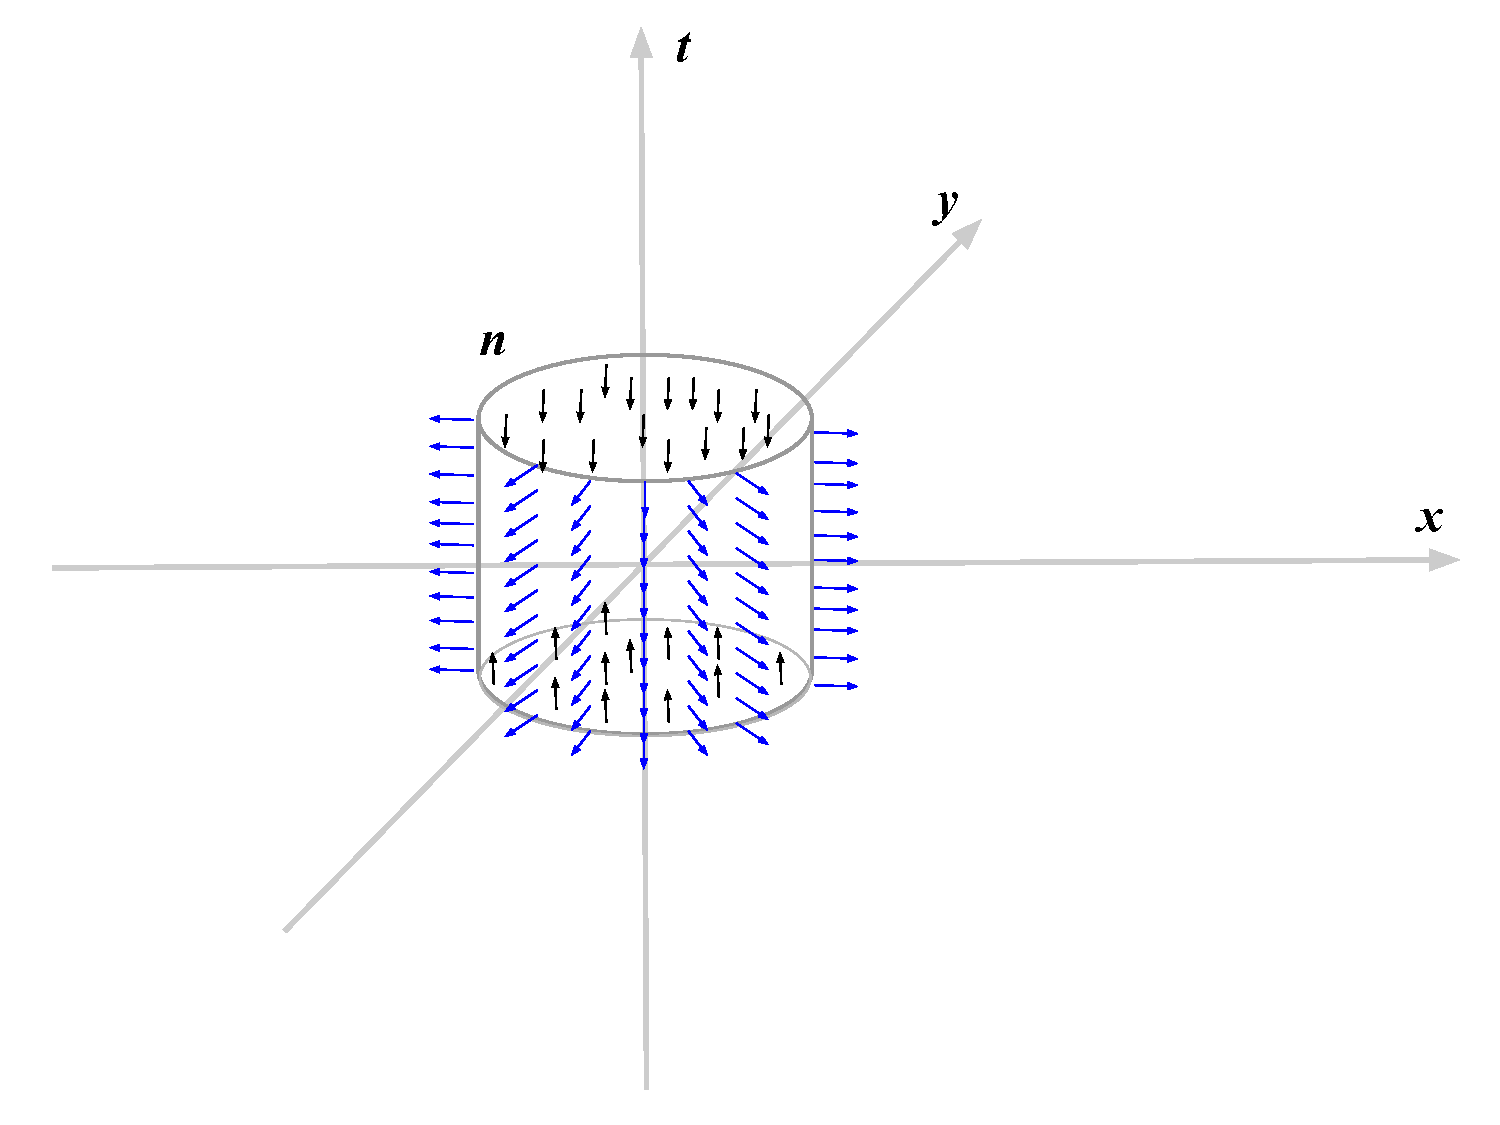
\includegraphics[scale=0.5]{figs/SpaceTimeNormal}
%\caption{Normal vectors to the oriented surface in spacetime. Blue arrows indicate spacelike vectors. Black arrows indicate timelike vectors.}
%\end{figure}
%
%In the context of Special Theory of Relativity the equation \ref{divergence-theorem} becomes
%\begin{equation}
%\label{divergence-theorem-special}
%\int_M \partial_\mu v^\mu d^4 x = \int_{\partial M} v^\mu dn_\mu.
%\end{equation} 
%
%\begin{theorem} (Relativistic Field Euler-Lagrange equations) If $$\bar{\delta} (S[M, \phi_0^\alpha]) = 0$$ for variation $\bar{\delta}$ with all partial derivatives $\partial_\mu \bar{\delta}\phi^\alpha$ and $\partial_\nu\partial_\mu \bar{\delta}\phi^\alpha$ infinitesimal of the first order and $\bar{\delta} \phi^\alpha$ vanishes on $\partial M$, then
%\begin{equation} 
% \cfrac{\partial \mathcal{L}}{\partial \phi^\alpha} - \partial_\mu \Pi^\mu_\alpha = 0
%\end{equation}
%for $\phi_0^\alpha$ on the interior of $M$.
%\end{theorem}   
%\begin{proof}
%Let $S = S[M, \phi_0^\alpha]$, then $\bar{\delta} S = \int_M \bar{\delta} \mathcal{L} d^4 x$. From (\ref{variation-lagrangian}) it follows that
%\begin{equation}
%\bar{\delta} S = \int_M \bigg(\cfrac{\partial \mathcal{L}}{\partial \phi^\alpha} - \partial_\mu \Pi^\mu_\alpha \bigg)\bar{\delta}\phi^\alpha d^4 x + \int_M\partial_\mu(\Pi^\mu_\alpha \bar{\delta}\phi^\alpha) d^4x.
%\end{equation}
%By Divergence Theorem (\ref{divergence-theorem-special}), we have
%\begin{equation}
%\int_M\partial_\mu(\Pi^\mu_\alpha \bar{\delta}\phi^\alpha) d^4x = \int_{\partial M} \Pi^\mu_\alpha \bar{\delta}\phi^\alpha dn_\mu = 0,
%\end{equation}
%because $\bar{\delta} \phi^\alpha$ vanishes on $\partial M$. Then
%\begin{equation}
%\bar{\delta} S = \int_M \bigg(\cfrac{\partial \mathcal{L}}{\partial \phi^\alpha} - \partial_\mu \Pi^\mu_\alpha \bigg)\bar{\delta}\phi^\alpha d^4 x.
%\end{equation}
%Since $\bar{\delta} S = 0$ and $\bar{\delta}\phi^\alpha$ is arbitrary enough, we have
%\begin{equation}
%\cfrac{\partial \mathcal{L}}{\partial \phi^\alpha} - \partial_\mu \Pi^\mu_\alpha = 0.
%\end{equation}
%\end{proof}
%
%For a given Lagrangian density $\mathcal{L} = \mathcal{L}(\phi^\alpha(x), \partial_\mu \phi^\alpha(x), x^\mu)$, consider small symmetry transformation of coordinates $\hat{x}^\mu = x^\mu + \delta_S x^\mu$.
%
%\begin{equation}
%\delta_S \mathcal{L} = \mathcal{L}(\phi^\alpha(\hat{x}), \partial_\mu \phi^\alpha(\hat{x}), \hat{x}^\mu) - \mathcal{L}(\phi^\alpha(x), \partial_\mu \phi^\alpha(x), x^\mu).
%\end{equation}
%
%Let's build a new field from the field $\phi^\alpha$.
%\begin{equation}
%\tilde{\phi}^\alpha(x) := \phi^\alpha(x + \delta_s x) = \phi^\alpha(x) + \partial_\nu \phi(x)\delta_s x^\nu.
%\end{equation}
%
%Let's write a new Lagrangian density
%\begin{equation}
%\tilde{\mathcal{L}}(\tilde{\phi}^\alpha(x), \partial_\mu\tilde{\phi}^\alpha(x), x) = \mathcal{L}(\tilde{\phi}^\alpha(x), \partial_\mu\tilde{\phi}^\alpha(x), x + \delta_S x).
%\end{equation}
%
%\begin{proposition}
%If
%\begin{equation} 
%\delta_S \mathcal{L} = \partial_\mu W^\mu(\phi, x) \delta \epsilon
%\end{equation}
% then $\phi^\alpha_0$ extremises $S[\phi, M]$ for $\phi = \phi^\alpha_0 + \bar{\delta}\phi^\alpha$ where $\bar{\delta}\phi^\alpha$ vanishes on $\partial M$ if and only if $\tilde{\phi}^\alpha_0$ extremises $\tilde{S}[\tilde{\phi}, M]$ for $\tilde{\phi} = \tilde{\phi}^\alpha_0 + \bar{\delta}\tilde{\phi}^\alpha$ where $\bar{\delta}\tilde{\phi}^\alpha$ vanishes on $\partial M$.
%\end{proposition}

\section{Sunday, 23 January 2022}

This is about alternative formulation of relativistic quantum theory, where we will introduce observables related to $4$-momentum. Energy operator will be then 

\begin{equation}
E\phi = i\hbar \cfrac{\partial}{\partial x^0} \phi,
\end{equation}

(Hamiltonian in this interpretation will not have meaning identical with energy operator but will be related exactly as you would expect from Schrödinger's equation $E\phi = H\phi$) and momentum as usual.

\begin{equation}
P_k\phi = - i\hbar \cfrac{\partial}{\partial x^k} \phi.
\end{equation}

Consequently, we will have $T$ time operator or $X_0$ if one likes.
\begin{equation}
T\phi = x_0\phi.
\end{equation}

Note that
\begin{equation}
[T, E] = -i\hbar{}.
\end{equation}

Indeed,
\begin{multline*}
\\
[T, E]\phi = (TE - ET)\phi = x_0 i\hbar\cfrac{\partial}{\partial x^0} \phi - i\hbar\cfrac{\partial}{\partial x^0}(x_0\phi)\\
\\ =  x_0 i\hbar\cfrac{\partial}{\partial x^0} \phi - i\hbar \phi - x_0 i\hbar\cfrac{\partial}
{\partial x^0} \phi
= - i\hbar \phi.
\\
\end{multline*}

The above is obviously a time-energy Heisenberg uncertainty principle. 

Note that we immediately get an invariance of uncertainty principle under Lorentz transformation. Assume $\beta\in (0, 1)$ is an arbitrary velocity ($c = 1$) and $\gamma = (1 - \beta^2)^{-1/2}$.  Let's take a Lorentz transformation of $4$-vector observables

\begin{equation}
X' = \gamma X - \beta\gamma T,
\end{equation}

\begin{equation}
T' = \gamma T - \beta \gamma X.
\end{equation} 

Let's take also Lorentz transformation of $4$-momentum observables

\begin{equation}
P_x' = \gamma P_x - \beta\gamma E,
\end{equation}

\begin{equation}
E' = \gamma E - \beta\gamma P_x.
\end{equation}

For this moment we may forget definitions of our operators. All that matters are their commutators $[X, P_x] = i\hbar$ and $[T, E] = -i\hbar$ and $[X, T] = [P_x, E] = [T, P_X] = [X, E] = 0$ (Note that commutation relations are analogous to Minkowski's metric tensor which corresponds nicely with why energy operator is defined with opposite sign than momentum operator).

Indeed,
\begin{equation}
[X', P'_x] = \gamma^2 [X, P_x] + \beta^2\gamma^2[T, E] = i\hbar\cfrac{1 - \beta^2}{1 - \beta^2} = i\hbar.
\end{equation}

\begin{equation}
[T', E'] = \gamma^2 [T, E] + \beta^2\gamma^2[X, P_x] = i\hbar \frac{\beta^2 - 1}{1 - \beta^2} = -i\hbar.
\end{equation}

Invariance of $[X, P_x] = i\hbar$ and $[T, E] = -i\hbar$ has fundamental meaning given the defining role of these commutators in quantum mechanics. We can express it that we got exactly the same quantum mechanics in each Lorentz frame of reference.

Interpretation of this formulation of quantum mechanics, which will give us the same results as at least classical quantum mechanics for non-relativistic case is following. We treat $\phi$ as a quantum state which describes the whole history of a particle. When we want to know what are the properties of the particle in time $t$ for a given frame of reference, we collapse state $\phi$ by projecting it on the subspace $\{\psi: T\psi = t\psi\}$, I. e, we first make an assumption that we have just measured time $T$ of the state $\phi$ an got measurement $t$, then we can do any other sort of things on the collapsed state to establish its property at time $t$.

\section{Sunday, 07 March 2022}

Let assume we have a group $U(\epsilon)$ of linear transformations of $\R^n$. Let $A$ be it's generator, i.e:

\begin{equation}
\cfrac{d}{d\epsilon} U(\epsilon)x \bigg|_{\epsilon=0} = A x.
\end{equation}

or using Einstein summation convention:

\begin{equation}
\cfrac{d}{d\epsilon} U(\epsilon)^\mu_\nu x^\nu \bigg|_{\epsilon=0} = A^\mu_\nu x^\nu.
\end{equation}

or in exponential form 
\begin{equation}
U(\epsilon) = e^{\epsilon A}.
\end{equation}

Consider transformation on $\phi: \R^n\to\C$ defined as
\begin{equation}
\big(\hat{U}(\epsilon)\phi\big)(x) := \phi(U(-\epsilon)x).
\end{equation}
Note that $\hat{U}(\epsilon)$ moves the shape of function $\phi$ against its domain exactly in the same direction as $U(\epsilon)$ transforms domain.
Note that
\begin{multline}\\
\cfrac{d}{d\epsilon} \big(\hat{U}(\epsilon)\phi\big)(x) \bigg|_{\epsilon=0} =
 \cfrac{d}{d\epsilon} \phi(U(-\epsilon)x) \bigg|_{\epsilon=0}\\
 = \partial_\mu \phi(U(-\epsilon)x) \cfrac{d}{d\epsilon} U(-\epsilon)^\mu_\nu x^\nu \bigg|_{\epsilon=0}
 = - \partial_\mu \phi(x) A^\mu_\nu x^\nu.
 \\
\end{multline}

Thus generator of $\hat{U}(\epsilon)$ denoted as $\hat{A}$ is given by
\begin{equation}
(\hat{A}\phi)(x) = - \partial_\mu \phi(x) A^\mu_\nu x^\nu.
\end{equation}

\section{Saturday, 26 November 2022}

Some considerations relevant to subsection \ref{fermi-golden-rule}

We will make now futher assumptions to simplify calculations. We will assume that perturbation is very slowly ``turned on'' in the past $t_0 \to -\infty$ and that there is ceratin fixed perturbation frequency $\omega$, so that $W(t) = e^{\eepsilon t}W e^{-i\omega t}$ (note that $\eepsilon$ is different small number than $\epsilon$), where $W$ is certain constant in time perturbation operator. Note also that such $W(t)$ is not self-adjoint. Purpouse of this will be explained later. If you feel uncomfortable with this, just set $\omega = 0$ for the time being.   

To make notation simpler use $\omega_{\beta\alpha} = E_\beta - E_\alpha$ and
$W_{\beta\alpha} = \bra{\phi_\beta}W\ket{\phi_\alpha}$.

Note that with above assumptions, we have

\begin{align*}
& \rho^{\gamma_n, \gamma_0}_n(t) = \int_{-\infty}^t ds_n \int_{-\infty}^{s_n} ds_{n - 1}\dots \int_{-\infty}^{s_2} ds_1 \int d\gamma_{n-1} \dots \int d\gamma_1 \\
& \prod_{k=1}^n \exp(is_k(\omega_{\gamma_k\gamma_{k - 1}} - \omega -i\eepsilon)) W_{\gamma_k \gamma_{k - 1}}.
\end{align*}

For fixed $\alpha = \gamma_0, \gamma_1, \dots, \gamma_{n-1}, \gamma_n = \beta$,
let's define
\begin{equation}
\sigma_{n,m}(t)[f] = \int_{-\infty}^t ds_n \int_{-\infty}^{s_n} ds_{n - 1}\dots \prod_{k=m + 1}^{n} \exp(is_k(\omega_{\gamma_k\gamma_{k - 1}} - \omega -i\eepsilon)) \int_{-\infty}^{s_{m + 1}} fds_m
\end{equation}

Note that
\begin{align*}
& \rho^{\gamma_n, \gamma_0}_n(t) = \int d\gamma_{n-1} \dots \int d\gamma_1 \\
& \prod_{k=1}^n W_{\gamma_k \gamma_{k - 1}}\sigma_{n,1}(t)[\exp(is(\omega_{\gamma_{1}\gamma_0} - \omega -i\eepsilon)))].
\end{align*}

Note the following basic properties of $\sigma_{n,m}(t)[f]$:

\begin{equation}
\begin{cases}
\sigma_{n,n}(t)[f] = \int_{-\infty}^t f(s) ds,\\
\sigma_{n,m}(t)[f] = \sigma_{n,m + 1}(t)[\exp(is(\omega_{\gamma_{m+1}\gamma_{m}} - \omega -i\eepsilon))\int^s_{\infty} f(s') ds'],
\end{cases}
\end{equation}

and thus

\begin{multline}
\sigma_{n,m}(t)[\exp(is(\omega_{\gamma_{m}\alpha} - m\omega -mi\eepsilon)))]\\
= \cfrac{-i}{\omega_{\gamma_{m}\alpha} - m\omega -im\eepsilon}\sigma_{n,m + 1}(t)[\exp(is(\omega_{\gamma_{m+1}\alpha} - (m+1)\omega -(m+1)i\eepsilon))].\\
\end{multline}

Hence

\begin{multline*}
\rho^{\beta, \alpha}_n(t) = \\(-i)^n \cfrac{e^{n\eepsilon t}e^{it(\omega_{\beta\alpha} - n\omega)}}{\omega_{\beta\alpha} - n\omega - ni\eepsilon}\int d\gamma_{n-1} \dots \int d\gamma_1 \prod_{k=1}^n W_{\gamma_k \gamma_{k - 1}} \prod_{k=1}^{n-1} \cfrac{1}{\omega_{\gamma_{k}\alpha} - k\omega -ik\eepsilon}. 
\end{multline*}

Let's give explicit formulas for $\omega = 0$:

\begin{equation}
\rho^{\beta, \alpha}_1(t) = -i \cfrac{e^{\eepsilon t}e^{it\omega_{\beta\alpha}}}{\omega_{\beta\alpha} - i\eepsilon}W_{\beta\alpha},
\end{equation}

\begin{equation}
\rho^{\beta, \alpha}_2(t) = -i \cfrac{e^{2\eepsilon t}e^{it\omega_{\beta\alpha}}}{\omega_{\beta\alpha} - i2\eepsilon}\int d \gamma \cfrac{ W_{\beta\gamma}W_{\gamma\alpha}}{\omega_{\gamma\alpha} - i\eepsilon}.
\end{equation}

\section{Friday, 30 December 2022}

A special case of Jordan's Lemma (not really important once you prove Jordan's Lemma).

\begin{lemma}
\label{cancel-half-circle}
Let $\Gamma_R$ be a path
\begin{equation}
\theta \mapsto Re^{i\theta} \text{ for } \theta\in[0, \pi].
\end{equation}
Let $f:\C \to \C$ be a masurable function on all $\Gamma_R$ for large enough $R$ and there exists $M > 0$ such that
\begin{equation}
\lim_{R\to\infty} \sup_{\Gamma_R} |f| < M.
\end{equation}
Then for any complex number $z\in \C$ and $a > 0$, we have
\begin{equation}
\lim_{R\to \infty} \int_{\Gamma_R} \cfrac{f(\gamma)}{\gamma + z}e^{ia\gamma}d\gamma = 0.
\end{equation} 
\end{lemma}
\begin{proof}
Note that $d\gamma = iRe^{i\theta} d\theta$, thus
\begin{equation}
\int_{\Gamma_R} \cfrac{f(\gamma)}{\gamma + z}e^{ia\gamma}d\gamma =
\int_0^\pi f(Re^{i\theta}) \cfrac{iRe^{i\theta}}{Re^{i\theta} + z} \exp(iaRe^{i\theta})d\theta.
\end{equation}
Note that for big enough $R$, we have
\begin{equation}
\big| f(Re^{i\theta})\big| < 2M
\end{equation}
and 
\begin{equation}
\bigg|  \cfrac{iRe^{i\theta}}{Re^{i\theta} + z} \bigg| < \bigg|  \cfrac{iRe^{i\theta}}{\frac{1}{2}Re^{i\theta}} \bigg| < 2.
\end{equation}
Thus
\begin{align*}
& \bigg| \int_{\Gamma_R} \cfrac{f(\gamma)}{\gamma + z}e^{ia\gamma}d\gamma \bigg| \leq
4M \int_0^\pi \big| \exp(iaR\cos\theta)\big| \exp(-aRsin\theta) d \theta = \\
& 4M \int_0^\pi \exp(-aRsin\theta) d \theta = 8M \int_0^{\pi/2} \exp(-aRsin\theta) d \theta.
\end{align*}

Note that for each $R > 0$ we have $\theta_R$ such that $\sin \theta_R = R^{-1/2}$.
Then, we have
\begin{equation}
\int_{\theta_R}^{\pi/2} \exp(-aRsin\theta) d \theta \leq \int_{\theta_R}^{\pi/2} \exp(-aR^{1/2}) d \theta = (\pi/2 - \theta_R) \exp(-aR^{1/2}),
\end{equation}
and
\begin{equation}
\int_0^{\theta_R} \exp(-aRsin\theta) d \theta \leq \theta_R.
\end{equation}
Hence we have
\begin{equation}
\int_0^{\pi/2} \exp(-aRsin\theta) d \theta \leq \theta_R + (\pi/2 - \theta_R) \exp(-aR^{1/2}) \xrightarrow[R \to \infty]{} 0.
\end{equation} 
\end{proof}

\begin{corollary}
\label{cancel-half-circle-cor}
The above lemma holds symmetrically for a path $\Gamma_R$
\begin{equation}
\theta \mapsto Re^{i\theta} \text{ for } \theta\in[\pi, 2\pi].
\end{equation}
and for $a < 0$.
\end{corollary}

The bellow fact is proven here more directly.

\begin{proposition}
\begin{equation}
\theta(a) = \lim\limits_{\epsilon\to 0^+} \cfrac{i}{2\pi} \int_{-\infty}^\infty  \cfrac{e^{-iax}}{x + i\epsilon} dx
\end{equation}
for $a\not=0$.
\end{proposition}
\begin{proof}
Take $a > 0$. Consider a path $\Gamma$ from $R$ to $-R$ closed by a half-circle $\Gamma_{-R}: \theta \mapsto Re^{i\theta}$ for $\theta\in[\pi, 2\pi]$. ($-R$ in $\Gamma_{-R}$ simply indicates that we take lower part of the cirle). Since $-i\epsilon$ belongs to the interior of $\Gamma$, by Theorem \ref{cauchy-convex}, we have


\begin{align*}
& e^{-a\epsilon} = \cfrac{1}{2\pi i} \int_\Gamma \cfrac{e^{-iax}}{x + i\epsilon} dx =
- \cfrac{1}{2\pi i} \int_{-R}^R \cfrac{e^{-iax}}{x + i\epsilon} dx + 
\cfrac{1}{2\pi i} \int_{\Gamma_{-R}} \cfrac{e^{-iax}}{x + i\epsilon} dx = \\
& \cfrac{i}{2\pi} \int_{-R}^R \cfrac{e^{-iax}}{x + i\epsilon} dx + 
\cfrac{1}{2\pi i} \int_{\Gamma_{-R}} \cfrac{e^{-iax}}{x + i\epsilon} dx.
\end{align*}
By Corollary \ref{cancel-half-circle}, we have
\begin{equation}
\lim_{R\to \infty} \cfrac{i}{2\pi} \int_{-R}^R \cfrac{e^{-iax}}{x + i\epsilon} dx = e^{-a\epsilon}.
\end{equation}
Thus
\begin{equation}
\lim\limits_{\epsilon\to 0^+} \cfrac{i}{2\pi} \int_{-\infty}^\infty  \cfrac{e^{-iax}}{x + i\epsilon} dx = 1.
\end{equation}

Now, take $a < 0$. Consider a new path $\Gamma$ from $-R$ to $R$ closed by a half-circle $\Gamma_{R}: \theta \mapsto Re^{i\theta}$ for $\theta\in[0, \pi]$. Since $-i\epsilon$ does not belong to the interior of $\Gamma$, by Theorem \ref{cauchy-convex}, we have
\begin{equation}
\cfrac{1}{2\pi i} \int_\Gamma \cfrac{e^{-iax}}{x + i\epsilon} dx = 0.
\end{equation}

Now, by Corollary \ref{cancel-half-circle-cor}, we have 
\begin{equation}
\lim_{R\to \infty} \cfrac{1}{2\pi i} \int_{\Gamma_{R}} \cfrac{e^{-iax}}{x + i\epsilon} dx = 0,
\end{equation}
hence
\begin{equation}
0 = \lim_{R\to \infty}\cfrac{1}{2\pi i} \int_{-R}^R \cfrac{e^{-iax}}{x + i\epsilon} dx = 
\cfrac{1}{2\pi i} \int_{-\infty}^\infty  \cfrac{e^{-iax}}{x + i\epsilon} dx.
\end{equation}
\end{proof}

\section{Sunday, 8 January 2023}

Assume we take a ket state parametrised in position coordicates $\ket{x_1, \dots, x_n}$. We have position and momentum operators defined as follows
\begin{align}
\label{diary-momentum-equation}
& \bra{x_1, \dots, x_n}P_k \ket{\phi} = -i\cfrac{\partial}{\partial x_k} \bra{x_1, \dots, x_n}\ket{\phi},\\
& \bra{x_1, \dots, x_n}Q_k \ket{\phi} = x_k \bra{x_1, \dots, x_n}\ket{\phi}.
\end{align}

It is easy to show commutation relation $[Q_{k'}, P_{k}] = i\delta_{k'k}$.

There is an interesting argument by Dirac (see \cite{dirac1981}[22]), that any observable $\Pi$ which has the same commutation relation with $Q_k$, namely for a chosen $k$
\begin{equation}
\label{diary-heisenber-uncertity-momentum}
[Q_{k'}, \Pi] = i\delta_{k'k},
\end{equation}
satisfies equation
\begin{equation}
\Pi = P_k + f(Q_1, \dots, Q_n)
\end{equation}
for some function $f$.
This comes from a very simple observation that $[Q_{k'}, \Pi - P_k] = 0$ for all $k'$, thus
by Theorem 2 from (see \cite{dirac1981}[19]), which states that observable which commutes with the complete set of commutable observables is a function on them, $\Pi - P_k$ must be a function of $Q_1, \dots, Q_n$. This is exactly what will hapen with canonical momentum and kinematic momentum in case of charged particle in magnetic field.

It is very importnat to remeber that (\ref{diary-heisenber-uncertity-momentum}) is not enough to get (\ref{diary-momentum-equation}) for $\Pi$.

\section{Manday, 9 January 2023}

Consider Weyl transform formula:
\begin{equation}
\hat{H} = \int \frac{dk}{2\pi} \cfrac{dx}{2\pi} e^{ikQ + ixP} \int dpdq e^{-ipx -ikq} H(p, q),
\end{equation}

where $H$ is just a function of real variables, $P$ is momentum operator and $Q$ is position operator.

To investigate how Weyl transform builds operator $\hat{H}$ from $H$ assume first that it is a monomial and put in through Corollary \ref{corollary-for-weyl-transform}. It is easy to see from it how it will act on multivariate polynomials and by extension on all their limit functions.

Let's represent the formula using our symmetric Fourier Transform as defined in Definition \ref{fourier}

\begin{equation}
\hat{H} = (2\pi)^{-1}\int dk dx e^{ikQ + ixP} \F(H)(x, k).
\end{equation}

It can be proven (see e.g. \cite{hall2013}[13]) that
\begin{equation}
e^{ikQ + ixP} = e^{ikx/2}e^{ikQ}e^{ixP}.
\end{equation}

Let's put this in.

\begin{align*}
& \hat{H} = (2\pi)^{-1}\int dk dx\, e^{ikx/2} \int dq \ket{q}\bra{q} e^{ikQ}e^{ixP} \int dp \ket{p}\bra{p}  \F(H)(x, k) = \\
& \int dk dx dp dq\,  e^{ikx/2} e^{ikq} e^{ipq} e^{ixp} \F(H)(x, k) \ket{q}\bra{p}
\end{align*}

Consider now:
\begin{align*}
& \bra{q_2} \hat{H} \ket{q_1} = (2\pi)^{-1} \int dk dx dp\,  e^{ikx/2} e^{ikq_2} e^{ipq_2} e^{ixp} \F(H)(x, k) (2\pi)^{-1/2}e^{-ipq_1} = \\
& (2\pi)^{-1/2} \int dk dx\,  e^{ikx/2} e^{ikq_2} \F(H)(x, k)
\delta(q_2 + x - q_1) = \\ 
& (2\pi)^{-1/2} \int dk \, e^{ik(q_1 - q_2)/2} e^{ikq_2} \F(H)(q_1 - q_2, k) = \\
& (2\pi)^{-1}  \int dk dp dq e^{ik(q_1 - q_2)/2} e^{ikq_2} e^{-ip(q_1 - q_2) -ikq} H(p, q) = \\
& \int dp dq\, \delta(\cfrac{q_1 - q_2}{2} + q_2 - q) e^{ip(q_1 - q_2)} H(p, q) = 
\int dp\, e^{ip(q_2 - q_1)} H(p, \cfrac{q_1 + q_2}{2}).
\end{align*}

We derived formula
\begin{equation}
\boxed{
\bra{q_2} \hat{H} \ket{q_1} = \int dp\, e^{ip(q_2 - q_1)} H(p, \cfrac{q_1 + q_2}{2})
}
\end{equation}

Using the above formula, we can derive path integral.

\begin{align*}
& \bra{y}e^{-it\hat{H}}\ket{x} \xleftarrow[n \to \infty]{} \bra{y}(I - \cfrac{it}{n}\hat{H})^n\ket{x} = \\
& \bra{y}\int dq_0 
\ket{q_0} \bra{q_0} \bigg( \prod_{k=1}^n  (I - i\Delta t\hat{H}) \int dq_k 
\ket{q_k} \bra{q_k}\bigg)\ket{x} = \\
& \int \prod_{k=1}^n dq_k dp_k\, \prod_{k=1}^n \bigg( e^{ip_k(q_{k-1} - q_k)} \big( 1 - i\Delta tH(p_k, \cfrac{q_{k-1} + q_k}{2})\big)\bigg) 
\bra{y}\ket{q_0}\bra{q_n}\ket{x},
\end{align*}
where $\Delta t = \cfrac{t}{n}$. We will assume (which should be proved more regorously) that since $\Delta t \to 0$ while $n\to \infty$, we can replace  $1 - i\Delta tH(p_k, \cfrac{q_{k-1} + q_k}{2})$ with $\exp\big(-i\Delta t H(p_k, \cfrac{q_{k-1} + q_k}{2})\big)$.

Continue then our calculation
\begin{align*}
& \bra{y}e^{-it\hat{H}}\ket{x} \xleftarrow[n \to \infty]{} \\
& \int \prod_{k=1}^n dq_k dp_k\, \prod_{k=1}^n
\exp\bigg(ip_k(q_{k-1} - q_k)- i\Delta t H(p_k, \cfrac{q_{k-1} + q_k}{2})\bigg)
\delta(y - q_0)\delta(q_n - x) = \\
& \int \prod_{k=1}^n dq_k dp_k\, 
\exp\bigg(i\Delta t \sum_{k=1}^n p_k(\cfrac{q_{k-1} - q_k}{\Delta t})- H(p_k, \cfrac{q_{k-1} + q_k}{2})\bigg)
\delta(y - q_0)\delta(q_n - x).
\end{align*}

Assuming that $q_0, q_1, \dots, q_n$ goes from $x$ to $y$ in reversed order, in the dense limit of discretisation:
\begin{equation}
\boxed{
\bra{y}e^{-it\hat{H}}\ket{x}  = 
\int_{\Omega} \mathcal{D} q \mathcal{D} p \exp \bigg(\int_0^t p \dot{q} - H(p, q) dt\bigg)
}
\end{equation} 

where $\mathcal{D} p \mathcal{D} q$ means path integration over phase space and $\Omega$ denotes a set of all paths where $q(0) = x, q(t) = y$ and $p$ is arbitrary.

\section{Manday, 16 January 2023}

Let $\alpha = \alpha^1, \dots, \alpha^k$ be a certain abstract parametrisation of a base $\ket{\alpha}$ of quantum states space. 
We will assume standard normalisation $\bra{\alpha}\ket{\alpha'} = \delta(\alpha - \alpha')$ Next, suppose $u(\epsilon)$ is
a one parameter group of symmetries (i.e $|\det u(\epsilon)| = 1$) on the space of these parameters. Let's define an operator
\begin{equation}
\hat{U}(\epsilon) \ket{\alpha}  \stackrel{def}{=} \ket{u(\epsilon) \alpha}.
\end{equation}

It follows from Subsection \ref{unitary-transformations} that $\hat{U}(\epsilon)$ is a group of unitary operators (i.e. $\hat{U}(\epsilon)\hat{U}^\dagger(\epsilon) = \hat{U}^\dagger(\epsilon)\hat{U}(\epsilon) = I$).

Let $G$ be an infinitesimal generator of group $u(\epsilon)$, i.e.
\begin{equation}
u(\epsilon) = e^{-i\epsilon G}.
\end{equation}

Note that, imaginary unit in the equation above is purely conventional. We can always get this equation simply by mupliplying by $i$ some real generator.

Assume $\ket{\phi}$ is an arbitrary quantum state. For infinitesimal $\Delta \epsilon$, we have $u(\Delta\epsilon) = I - i\Delta\epsilon G$, then
\begin{equation}
\label{infinitesimal-move-in-symmetrybra}
\bra{\alpha} \hat{U}^{\dagger}(\Delta \epsilon)\ket{\phi} = \bra{\alpha - i\Delta\epsilon G\alpha}\ket{\phi}.
\end{equation}
Assume that $\hat{G}$ is a generator of $\hat{U}(\epsilon)$, i.e.
\begin{equation}
\hat{U}(\epsilon) = e^{-i\epsilon \hat{G}}.
\end{equation}
With infinitesimal $\Delta \epsilon$, we have $\hat{U}(\Delta \epsilon) = I - i\Delta\epsilon \hat{G}$. From this it is easy to show that $\hat{G} = \hat{G}^\dagger$. 
Now, from (\ref{infinitesimal-move-in-symmetrybra}) we have
\begin{align*}
& \bra{\alpha} I + i\Delta\epsilon \hat{G} \ket{\phi} = \bra{\alpha -i \Delta\epsilon G\alpha}\ket{\phi},\\
& i \Delta\epsilon \bra{\alpha} \hat{G}\ket{\phi} = \bra{\alpha -i \Delta\epsilon G\alpha}\ket{\phi} - \bra{\alpha}\ket{\phi}.
\end{align*} 

Let $\Delta \alpha = -i \Delta\epsilon G\alpha$. Then we have

\begin{align*}
& i \Delta\epsilon \bra{\alpha} \hat{G}\ket{\phi} = \bra{\alpha + \Delta\alpha}\ket{\phi} - \bra{\alpha}\ket{\phi},\\
& i \Delta\epsilon \bra{\alpha} \hat{G}\ket{\phi} = \cfrac{\partial}{\partial \alpha} \bra{\alpha}\ket{\phi} \cdot \Delta\alpha,\\
& i \Delta\epsilon \bra{\alpha} \hat{G}\ket{\phi} = -i \Delta \epsilon \cfrac{\partial}{\partial \alpha}  \bra{\alpha}\ket{\phi} \cdot G\alpha.
\end{align*}

Hence
\begin{equation}
\label{symmetry-generator-to-observable}
\boxed{
\bra{\alpha} \hat{G}\ket{\phi} = - \cfrac{\partial}{\partial \alpha}  \bra{\alpha}\ket{\phi} \cdot G\alpha
}
\end{equation}

Equation (\ref{symmetry-generator-to-observable}) shows us how to create an observable 
from symmetry generator defined in the space of parameters of base states. In this sense we can treat $\hat{\cdot}$ as map transforming generators to observables.

Let's assume we have two symmetry generators $A$ and $B$, which are linear opertors in space of parameters.
Let's do the following computation
\begin{align*}
& \bra{\alpha} \hat{A}\hat{B} \ket{\phi} = - \cfrac{\partial}{\partial \alpha^i}  
 \bra{\alpha} \hat{B} \ket{\phi} (A\alpha)^i = \\
&  \cfrac{\partial}{\partial \alpha^i} 
\bigg( \cfrac{\partial}{\partial \alpha^j} \bra{\alpha}\ket{\phi} (B\alpha)^j\bigg) (A\alpha)^i = \\
&  \bigg(\cfrac{\partial}{\partial \alpha^i} \cfrac{\partial}{\partial \alpha^j} \bra{\alpha}\ket{\phi} (B\alpha)^j + \cfrac{\partial}{\partial \alpha^j} \bra{\alpha}\ket{\phi} \cfrac{\partial}{\partial \alpha^i}(B\alpha)^j\bigg) (A\alpha)^i.
\end{align*}

Applying the above symmetrically we get
\begin{align*}
& \bra{\alpha} [\hat{A}, \hat{B}] \ket{\phi} = \cfrac{\partial}{\partial \alpha^j} \bra{\alpha}\ket{\phi} \cfrac{\partial}{\partial \alpha^i}(B\alpha)^j (A\alpha)^i 
- \cfrac{\partial}{\partial \alpha^j} \bra{\alpha}\ket{\phi} \cfrac{\partial}{\partial \alpha^i}(A\alpha)^j (B\alpha)^i = \\
& \cfrac{\partial}{\partial \alpha^j} \bra{\alpha}\ket{\phi}
\bigg(
 \cfrac{\partial}{\partial \alpha^i}(B\alpha)^j (A\alpha)^i 
- \cfrac{\partial}{\partial \alpha^i}(A\alpha)^j (B\alpha)^i
\bigg) = \\
& \cfrac{\partial}{\partial \alpha^j} \bra{\alpha}\ket{\phi}
\bigg(
 \cfrac{\partial}{\partial \alpha^i}(B^j_m\alpha^m) (A^i_n\alpha^n) 
- \cfrac{\partial}{\partial \alpha^i}(A^j_m \alpha^m) (B^i_n\alpha^n)
\bigg) = \\
& \cfrac{\partial}{\partial \alpha^j} \bra{\alpha}\ket{\phi}
\bigg(
 B^j_i A^i_n\alpha^n 
- A^j_iB^i_n\alpha^n
\bigg) = - \cfrac{\partial}{\partial \alpha} \bra{\alpha}\ket{\phi} \cdot [A, B]\alpha.
\end{align*}

We showed
\begin{equation}
\boxed{
\bra{\alpha} [\hat{A}, \hat{B}] \ket{\phi} = - \cfrac{\partial}{\partial \alpha} \bra{\alpha}\ket{\phi} \cdot [A, B]\alpha
}
\end{equation}

Hence, we have $\widehat{[A, B]} = [\hat{A}, \hat{B}]$. 
Which means that limear generators of symmetry group and induced observables form isomorphic Lie algebras.

\section{Sunday, 22 January 2023}

I would like to give a maximal genralisation of the fact showed above.
Let $\Omega$ and $\Sigma$ be two linear spaces both with vector multiplication, where  scalar multiplication, addition are continuous in a product and vector multiplication is seperatelly continous. Assume that we can reasonably define derivative in at least Gateaux sense for $F: \Theta\to\Sigma$, where $\Theta$ is certain open set in $\Omega$ (if $\Theta$ is a proper subset of $\Omega$, we need to assume that topology is locally convex).

\begin{equation}
\nabla F(\omega; \Delta\omega) \stackrel{def}{=} \lim_{\epsilon\to 0}\cfrac{F(\omega + \epsilon\Delta\omega) - F(\omega)}{\epsilon}.
\end{equation}

Let $C^1(\Theta,\Sigma)$ denote all mapings with continous derivaties at least in a sense which guarantees
\begin{equation}
F(\omega + \Delta \omega) - F(\omega) = \int_0^1 \nabla F (\omega + \tau\Delta\omega; \omega) d\tau
\end{equation}

and that mapping $\nabla F(\cdot; \Delta\omega)$ is continuous.

\begin{lemma} If $F\in C^1(\Theta,\Sigma)$, then
$\nabla F(\omega; \cdot)$ is linear for any $\omega\in\Theta$.
\end{lemma}
\begin{proof}
We have $\nabla F(\omega; a\Delta\omega) = a \nabla F(\omega; \Delta\omega)$ directly from definition.

Consider 
\begin{align*}
& \epsilon^{-1}(F(\omega + \epsilon\Delta\omega_1 + \epsilon\Delta\omega_2) - F(\omega)) = \\
& \epsilon^{-1}(F(\omega + \epsilon\Delta\omega_1 + \epsilon\Delta\omega_2) - F(\omega + \epsilon\Delta\omega_1) + F(\omega + \epsilon\Delta\omega_1) - F(\omega)) = \\
& \epsilon^{-1} \bigg(\int_0^1 \nabla F (\omega + \epsilon\Delta\omega_1 + \tau\epsilon \Delta\omega_2; \epsilon\Delta \omega_2) d\tau + \\
& \int_0^1 \nabla F (\omega + \tau\epsilon\Delta\omega_1; \epsilon\Delta \omega_1) d\tau\bigg) \xrightarrow[\epsilon \to 0]{} \nabla F (\omega; \Delta \omega_1) + \nabla F (\omega; \Delta \omega_2).
\end{align*}
\end{proof}

For $F\in C^1(\Theta,\Sigma)$, since we have linearity, we will write $\nabla F(\omega)\cdot \Delta\omega = \nabla F(\omega; \Delta\omega)$.

Assume that we have $U\in C^1(\Theta,\Sigma)$ such that $U(\omega_1)U(\omega_2) = U(\omega_1\omega_2)$ for $\omega_1, \omega_2, \omega_1\omega_2\in\Theta$. With fixed $U$ we can define operator $\hat{\cdot}: \Omega\to\Sigma$ and $U(\mathfrak{e}) = \mathfrak{e}$, where $\mathfrak{e}$ is a group unity and $\mathfrak{e}\in\Theta$.

\begin{definition} For $\omega\in \Omega$
\begin{equation}
\hat{\omega} \stackrel{def}{=} \lim_{\epsilon \to 0} \cfrac{U(\mathfrak{e} + \epsilon \omega) - \mathfrak{e}}{\epsilon}.
\end{equation}
\end{definition}

\begin{corollary}
\begin{equation}
\hat{\omega} = \nabla U(\mathfrak{e})\cdot \omega.
\end{equation}
\end{corollary}


\begin{theorem}
\label{general-lie-transition}
For $\omega_1, \omega_2\in \Omega$, we have 
\begin{equation}
\widehat{[\omega_1, \omega_2]} = [\hat{\omega}_1, \hat{\omega}_2].
\end{equation}
\end{theorem}
\begin{proof}
Consider
\begin{align*}
& \bigg(\cfrac{U(\mathfrak{e} + \epsilon_1 \omega_1) - \mathfrak{e}}{\epsilon_1}\bigg)
\bigg(\cfrac{U(\mathfrak{e} + \epsilon_2 \omega_2) - \mathfrak{e}}{\epsilon_2}\bigg) = \\
& (\epsilon_1\epsilon_2)^{-1}\big(
U(\mathfrak{e} + \epsilon_1\omega_1 + \epsilon_2\omega_2 + \epsilon_1\epsilon_2 \omega_1\omega_2)
- U(\mathfrak{e} + \epsilon_1 \omega_1) - U(\mathfrak{e} + \epsilon_2 \omega_2) + \mathfrak{e}
\big).
\end{align*}

applying the above symmetrically, we get
\begin{align*}
& \bigg[\cfrac{U(\mathfrak{e} + \epsilon_1 \omega_1) - \mathfrak{e}}{\epsilon_1},
\cfrac{U(\mathfrak{e} + \epsilon_2 \omega_2) - \mathfrak{e}}{\epsilon_2}\bigg] = \\
& (\epsilon_1\epsilon_2)^{-1} \big(
U(\mathfrak{e} + \epsilon_1\omega_1 + \epsilon_2\omega_2 + \epsilon_1\epsilon_2 \omega_1\omega_2)
- U(\mathfrak{e} + \epsilon_1\omega_1 + \epsilon_2\omega_2 + \epsilon_1\epsilon_2 \omega_2\omega_1\big) = \\
& (\epsilon_1\epsilon_2)^{-1} \big(
U(\mathfrak{e} + \epsilon_1\omega_1 + \epsilon_2\omega_2 + \epsilon_1\epsilon_2 \omega_2\omega_1 + \epsilon_1\epsilon_2[\omega_1, \omega_2])
- U(\mathfrak{e} + \epsilon_1\omega_1 + \epsilon_2\omega_2 + \epsilon_1\epsilon_2 \omega_2\omega_1)\big) = \\
& (\epsilon_1\epsilon_2)^{-1} \int_0^1 \nabla U(\mathfrak{e} + \epsilon_1\omega_1 + \epsilon_2\omega_2 + \epsilon_1\epsilon_2 \omega_2\omega_1) \cdot \epsilon_1\epsilon_2[\omega_1, \omega_2] = \\ 
& \int_0^1 \nabla U(\mathfrak{e} + \epsilon_1\omega_1 + \epsilon_2\omega_2 + \epsilon_1\epsilon_2 \omega_2\omega_1) \cdot [\omega_1, \omega_2] \xrightarrow[\epsilon_1, \epsilon_2 \to 0]{} 
\nabla U(\mathfrak{e}) \cdot [\omega_1, \omega_2].
\end{align*}
\end{proof}

Note that for the above theorem vector multiplication associativity is not required. We used only distributive property and $a (\omega_1\omega_2) = (a\omega_1)\omega_2 = \omega_1(a\omega_2)$ property.

\subsection{Application to Quantum Mechanics}

Assume that $\Omega$ is as above. Let $\mathcal{X}$ be a space of quantum states and $L(\mathcal{X})$ a space of linear operators on $\mathcal{X}$. Let $U\in C^1(\Theta, L(\mathcal{X}))$ be a family of unitary operators, which preserves multiplication, where $\Theta$ is an open neighbourhood of $\mathfrak{e}$.

\begin{definition} Let $-i\omega\in \Omega$.
\label{general-observable-definition}
\begin{equation}
O_\omega \stackrel{def}{=} i\lim_{\epsilon \to 0} \cfrac{U(\mathfrak{e} - i\epsilon \omega) - I}{\epsilon}.
\end{equation}
\end{definition}

\begin{proposition}
If $\omega\in \Omega$, then $O_\omega^\dagger = O_\omega$.
\end{proposition}
\begin{proof}
We will follow the bellow reasoning assuming that $\epsilon^2$ vanishes (it is a teachnicality to rewrite it to mathematically correct proof).
\begin{equation}
U(\mathfrak{e} - i\epsilon \omega)U(\mathfrak{e} + i\epsilon \omega) = U(\mathfrak{e} + \epsilon^2 \omega^2) = I.
\end{equation}
Thus $U^\dagger(\mathfrak{e} - i\epsilon \omega) = U(\mathfrak{e} + i\epsilon \omega)$. Hence,
\begin{align*}
O^\dagger_\omega = -i \cfrac{U(\mathfrak{e} + i\epsilon \omega) - I}{\epsilon} = i \cfrac{U(\mathfrak{e} - i\epsilon \omega) - I}{\epsilon} = O_\omega. 
\end{align*}
\end{proof}
\begin{proposition}
\label{general-lie-transition-quantum}
Let $-i\omega_1, -i\omega_2 \in \Omega$, then
\begin{align}
& O_{i\mathfrak{e}}  = I,\\
& O_{a_1\omega_1 + a_2\omega_2} = a_1 O_{\omega_1} + a_2 O_{\omega_2},\\
& [O_{\omega_1}, O_{\omega_2}] = O_{[\omega_1, \omega_2]}.
\end{align}
\end{proposition}
\begin{proof}
Follows from Theorem \ref{general-lie-transition}.
\end{proof}

Let's again, similary like on Monday, 16 January 2023, consider a special case where for a certain parametrisation $\alpha = \alpha^1, \dots, \alpha^k$ of a base $\ket{\alpha}$ of quantum states space with $\bra{\alpha}\ket{\alpha'} = \delta(\alpha - \alpha')$, we defined a family of unitary operators $\hat{U}$ parametrised by symmetries in parametrisation:
\begin{equation}
\hat{U}(u)\ket{\alpha} = \ket{u(\alpha)}.
\end{equation}

Take certain infinitesimal symmetry with generator $G$. Hence,
\begin{equation}
\hat{U}(I - i\epsilon G)\ket{\alpha} = \ket{\alpha - i\epsilon G\alpha}.
\end{equation}
On the other hand $I - i\epsilon O_G = \hat{U}(I - i\epsilon G)$. Thus
\begin{equation}
I - i\epsilon O_G\ket{\alpha} = \ket{\alpha - i\epsilon G\alpha}
\end{equation}
and
\begin{equation}
\bra{\alpha} I + i\epsilon O_G\ket{\phi} = \bra{\alpha - i\epsilon G\alpha}\ket{\phi}.
\end{equation}
Following similar reasoning which leads to \ref{symmetry-generator-to-observable} we will get analogously
\begin{equation}
\bra{\alpha} O_G \ket{\phi} = - \cfrac{\partial}{\partial \alpha}  \bra{\alpha}\ket{\phi} \cdot G\alpha.
\end{equation}

Now, the result of that day 
\begin{equation}
\bra{\alpha} [O_A, O_B] \ket{\phi} = - \cfrac{\partial}{\partial \alpha} \bra{\alpha}\ket{\phi} \cdot [A, B]\alpha
\end{equation}

is simply a corollary from Proposition \ref{general-lie-transition-quantum}.
\end{document}

